%: ----------------------- sigex file header -----------------------
\chapter{Vacuum Enhanced Mixing}
\label{sec:chameleons}

% the code below specifies where the figures are stored
\ifpdf
    \graphicspath{{chameleons}{chameleons/figures/PDF/}{chameleons/figures/}}
\else
    \graphicspath{{chameleons/figures/EPS/}{chameleons/figures/}}
\fi

% ----------------------------------------------------------------------
% ----------------------- chameleons content -------------------------
% ----------------------------------------------------------------------
%\section{Modified Vacuum Mixing}
Considered here is a novel phenomenological theory that modifies the solar
neutrino survival probability.
Whereas many theories of modified neutrino mixing alter the way neutrinos
interact with matter, similar to standard matter enhanced-mixing,
here we consider a modification to neutrino mixing in areas of very low matter
density.
 Motivations for a potential with strength inversely related to local matter
density is considered in Sec.~\ref{sec:motivations}.
The effect a potential of this form is might have on neutrino
mixing is parameterized as follows
\begin{equation}
H = UM^{2}U^{\dagger} + A_{\mathrm{vac}}\text{,}
\end{equation}
where $A_{\mathrm{vac}}$ represents a potential only significant in regions
of near-zero matter density.
$A_{\mathrm{vac}}$ is given by
\begin{equation}
A_{\mathrm{vac}} =
\begin{bmatrix}
    A_{\mathrm{e}} & 0 & 0  \\
    0 &  A_{\mathrm{\mu}} & 0  \\
    0 & 0 &  A_{\mathrm{\tau}}  \\
\end{bmatrix}\text{.}
\end{equation}
Each diagonal entry represents a potential felt in the vacuum
by the neutrino of the given flavor state.
This parameterization can be simplified somewhat by subtracting off
an identity like term.
\begin{equation}
A_{\mathrm{vac}}^{\prime} =
\begin{bmatrix}
    A_{\mathrm{e}} & 0 & 0  \\
    0 &  A_{\mathrm{\mu}} & 0  \\
    0 & 0 &  A_{\mathrm{\tau}}  \\
\end{bmatrix} - 
\begin{bmatrix}
    A_{\mathrm{\tau}} & 0 & 0  \\
    0 &  A_{\mathrm{\tau}} & 0  \\
    0 & 0 &  A_{\mathrm{\tau}}  \\ 
\end{bmatrix} 
= 
\begin{bmatrix}
    A_{\mathrm{e}}^{\prime} & 0 & 0  \\
    0 &  A_{\mathrm{\mu}}^{\prime} & 0  \\
    0 & 0 &  0  \\ 
\end{bmatrix}  
\end{equation}
This makes no difference because neutrino mixing is only effected by differences
between the neutrino states, so an identity-like matrix can always be subtracted
from the mixing Hamiltonian without effecting the result.

In this model mixing is described by standard MSW-LMA mixing in areas of
non-negligible matter density, and by the modified vacuum mixing potential
in areas of near zero matter density.
In areas where the matter effect on neutrinos is negligible but the local
matter density is non-zero, the mixing is best described a standard
vacuum mixing potential, \textit{i.e.} $H = UM^{2}U^{\dagger}$.
A model like this is desirable because it allows for the mixing of solar neutrinos, which
travel for a signifiant distance in the vacuum of space between the Sun and Earth,
to be modified, while not effecting neutrino mixing observed by terrestrial neutrino experiments.

Nearly all detected neutrino sources, neutrinos are produced, propagate through
 and detected are detected in areas of relatively high matter density
The exception to this is supernova neutrinos observed by from SN1987A~\citep{kamiokande_sn, imb_sn, baksan_sn},
and neutrinos detected by the IceCube experiment from a blazar~\citep{icecube_blazar}.
Neither of these datasets are sufficient to make statements
about neutrino mixing though.
Ultra-high energy neutrinos from the GZK production process~\citep{gzk} would be an useful
source for constraining this model, as GZK neutrinos not only travel through
significant distances in vacuum, they're also produced in vacuum.
However, neutrinos from the GZK process have not yet been detected by
any experiments.
And so, solar neutrinos are the only currently available source
of neutrinos that are sensitive to this model.

\section{Motivation}
\label{sec:motivations}
There are broadly two motivating factors behind a modified vacuum mixing model.
The first is the tension in between solar neutrino measurements and 
the KamLAND reactor neutrino measurement of $\Delta m^{2}_{21}$.
This tension is discussed in detail in Sec.~\ref{sec:dm21_tension}.
While the tension could be the result of statistical fluctuations or un-modelled
systematic effects, the flatness of observed solar survival probability and
unexpectedly large day-night asymmetry both independently prefer lower values
for $\Delta m^{2}_{21}$.
This motivates considerations of what physics might effect the solar survival
probability and not the KamLAND result.
Unexpected effects from the high density long baseline solar environment provide a neat answer.
Similarly unexpected effects from a near zero matter density environment
provides an explanation for the observed tension between the KamLAND and solar
results.
Some of the existing ideas for non-standard interactions in the Sun are discussed
in Sec.~\ref{sec:nsi}

The second motivating factor is that there exists theories that
suggest a potential in empty space across large distance scales may be the source
of the observed expansion of the universe~\cite{khoury_chameleons}.
This new potential is referred to as a ``chameleon'' force because it
is screened by the local matter around it, and so it ``blends in'' in
areas of relatively high matter density.
But in empty space the potential is much stronger and thus able to provide
a source of energy for the observed expansion of the universe.
The chameleon theory for dark energy could also provide a neutrino flavor dependent
potential that effects the oscillation of neutrinos in areas of very low matter
density.
The chameleon theory for dark energy here only provides a phenomenological basis
for considering modified vacuum neutrino mixing. The model proposed here is
not necessarily dependent on the chameleon dark energy theory, or vice versa.
This relationship is similar to how Mass Varying Neutrino (MaVaN) models
for neutrino oscillation are motivated by acceleron theories for dark energy,
but not specifically required~\cite{mavans_cosmology}.


\section{Measurements of \textbf{$\Delta m^{2}_{21}$}}
\label{sec:dm21_tension}
The current global best fit value for  $\Delta m^{2}_{21}$ and
$\theta_{12}$ comes
primarily from a combined fit to solar neutrino data from SNO
and Super-K and Borexino, and reactor neutrino data from KamLAND\@.
These fits have produced the values
\begin{equation}
    \Delta m^{2}_{21} = 7.39^{+0.21}_{-0.21}\times10^5 \text{eV}^{2}
\end{equation}
\begin{equation}
    \sin^2\theta_{12} = 0.310^{+0.013}_{-0.012}\text{.}
\end{equation}
However, KamLAND has much better sensitivity to $\Delta m^{2}_{21}$
than the combined SNO and Super-K result, so the best fit value for
$\Delta m^{2}_{21}$ comes almost exclusively from the KamLAND
reactor neutrino measurements.
\begin{figure}[htbp]
    \centering
    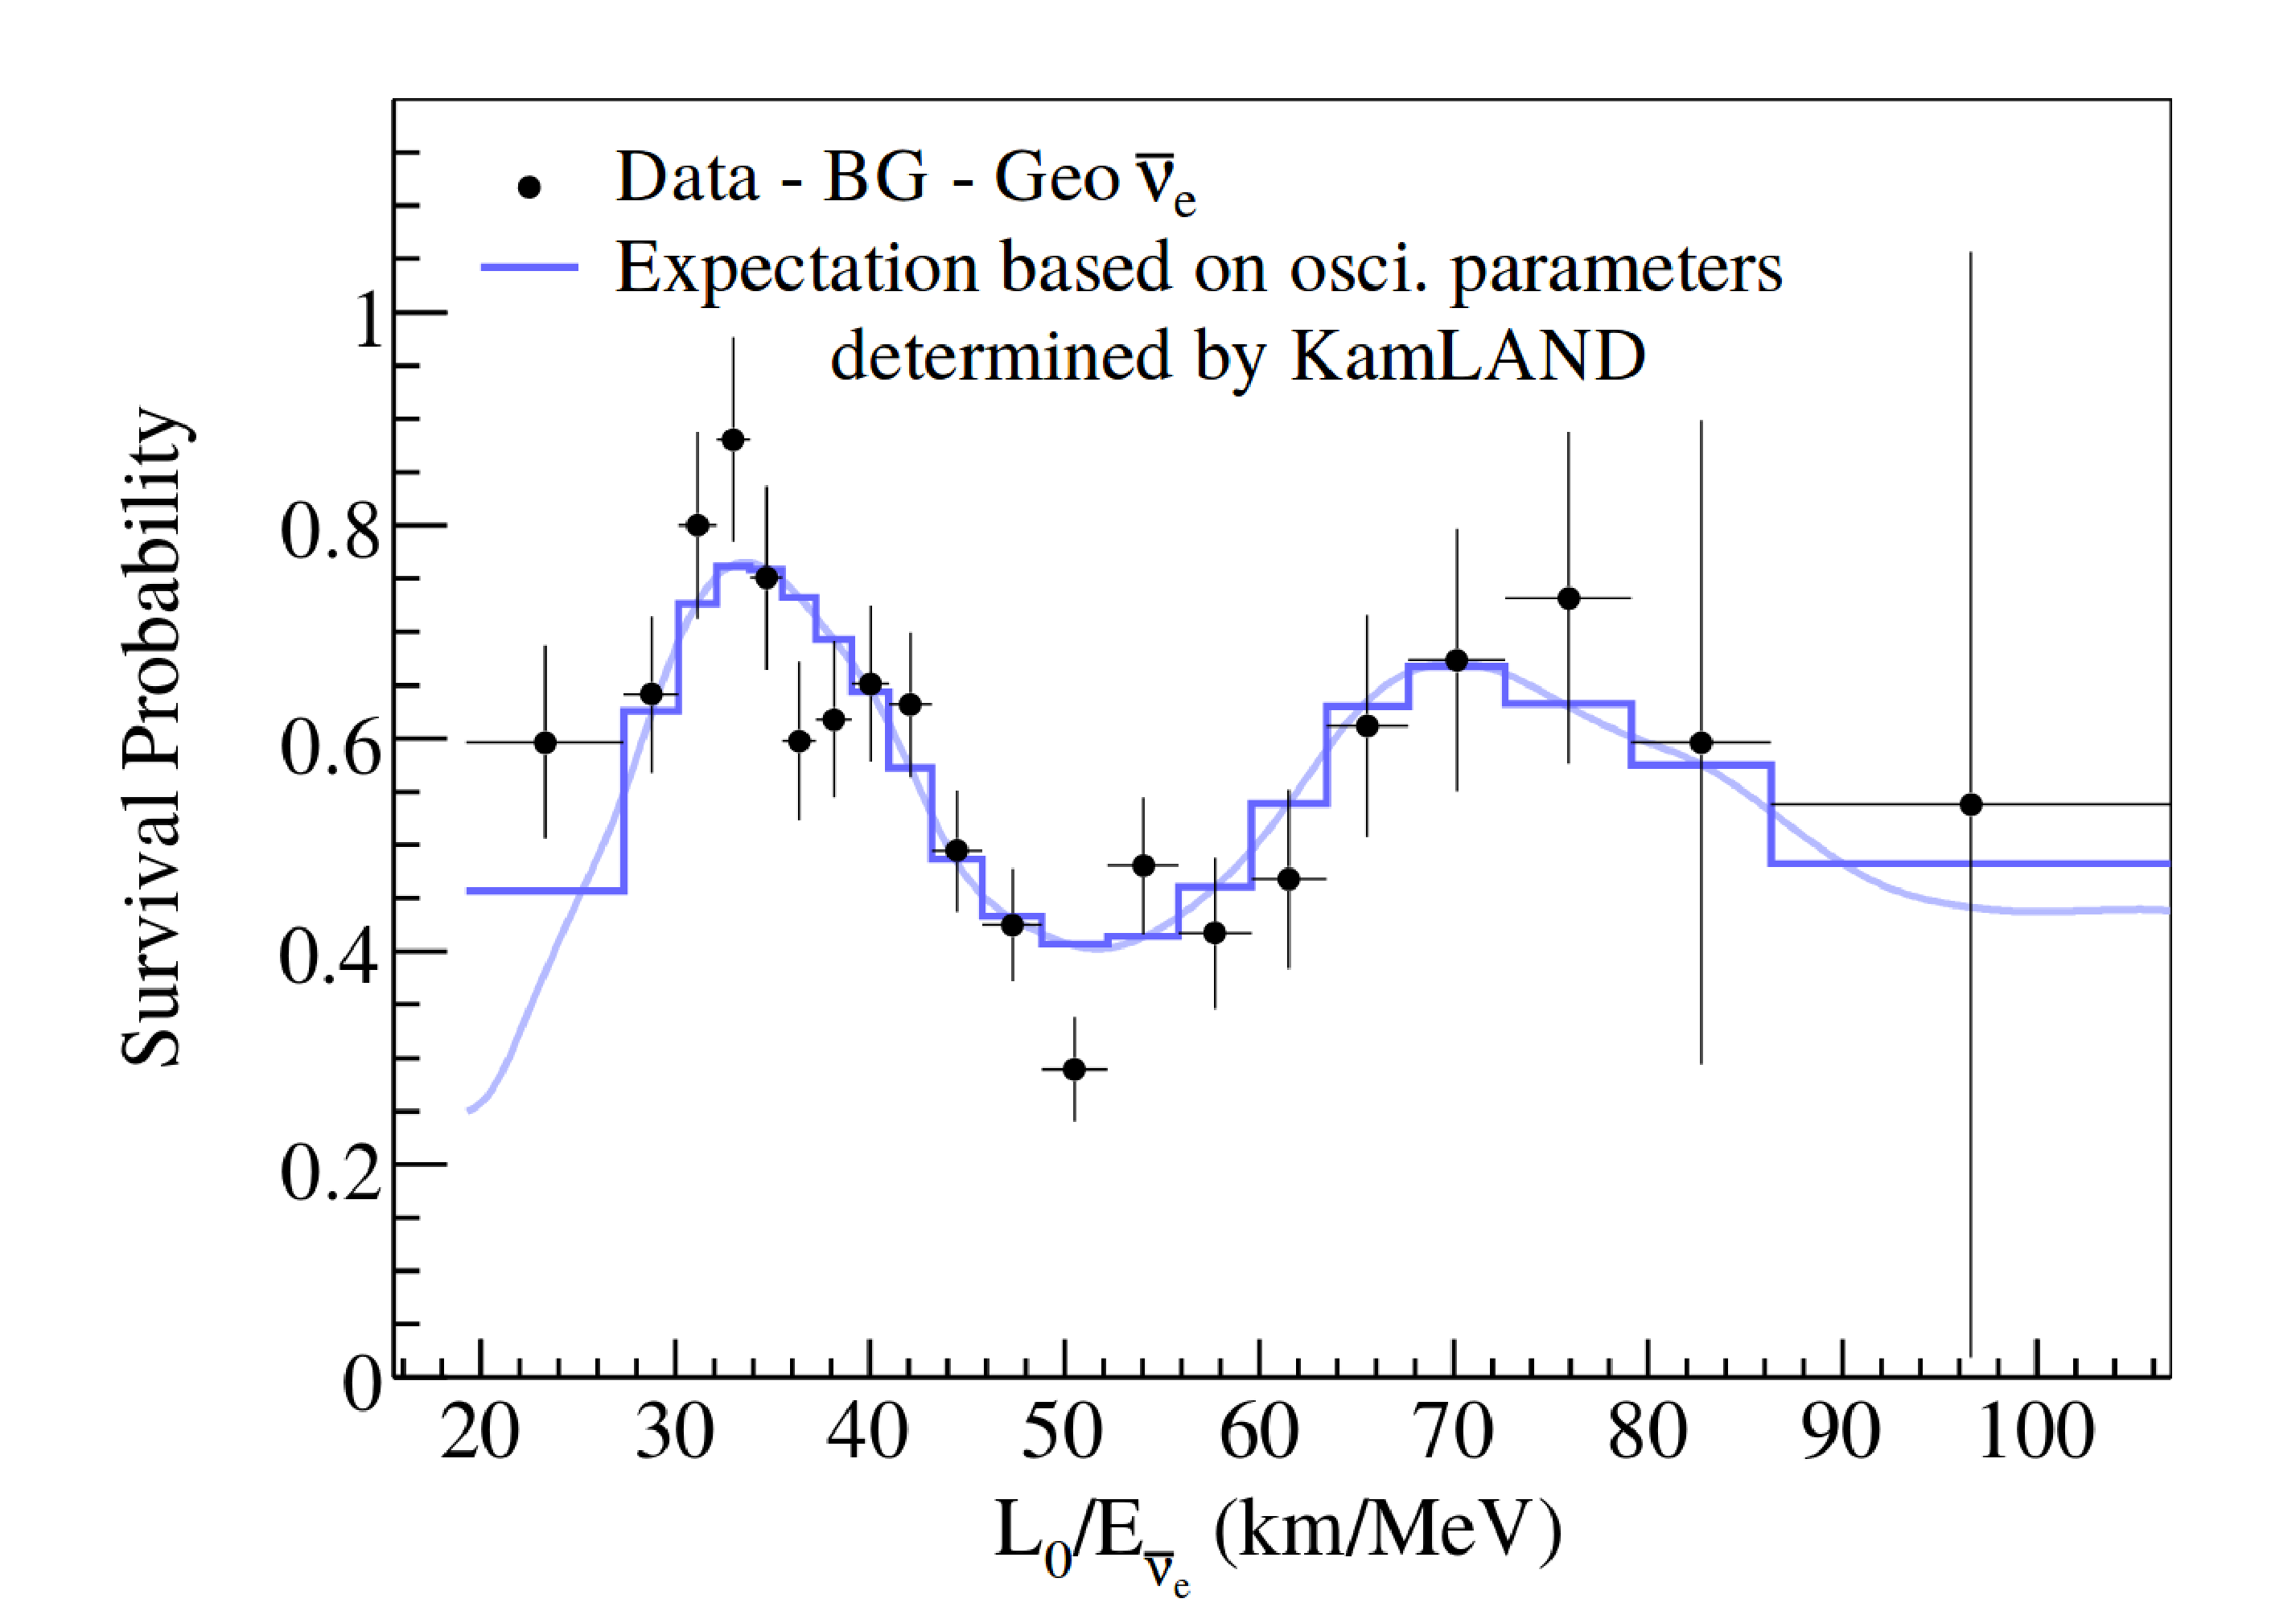
\includegraphics[width=\textwidth]{kamland_oscillation}
    \caption[]{}
    \label{fig:kamland_oscillation}
\end{figure}
The KamLAND measurement is discussed briefly in Sec~\ref{sec:kamland}.
The precision of their measurement comes from the fact that $\Delta m^{2}_{21}$
adjusts the ``wavelength'' in energy of oscillations in their observed
reactor neutrino spectrum.
Figure~\ref{fig:kamland_oscillation} shows KamLAND's observed oscillation
spectrum and best fit.

\begin{figure}[htbp]
    \centering
    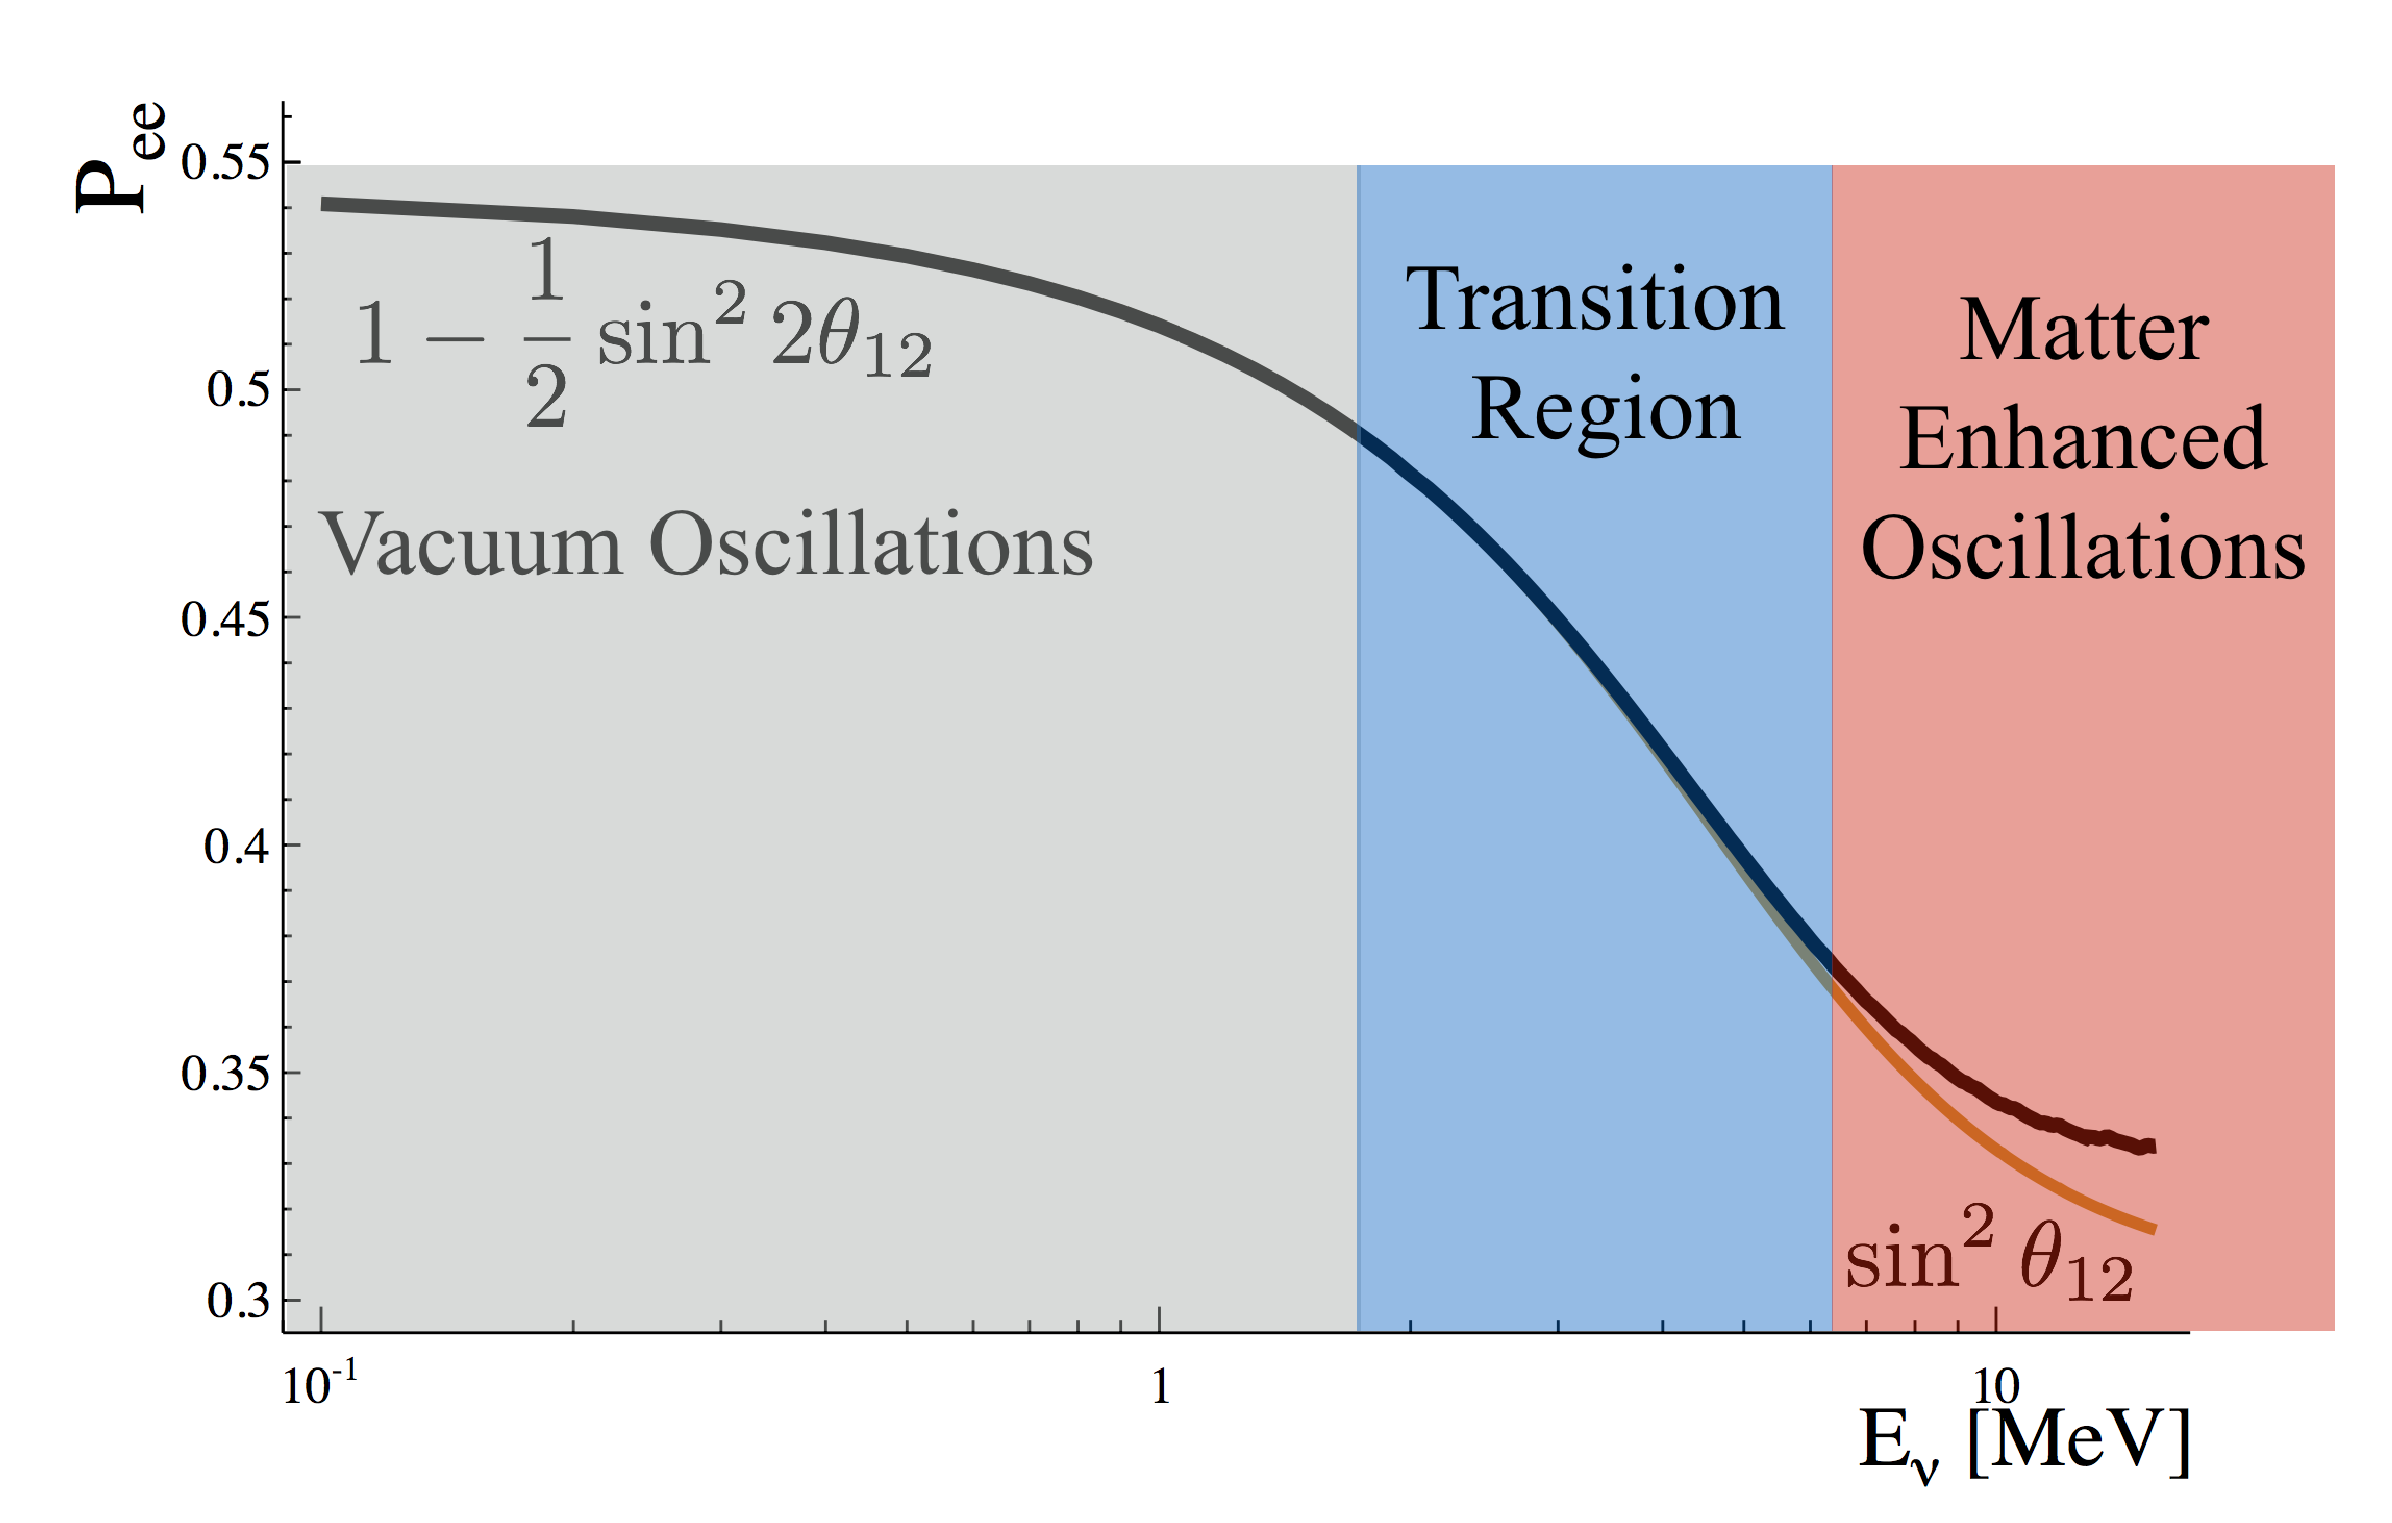
\includegraphics[width=0.78\textwidth]{labelled_survival_probability}
    \caption[]{}
    \label{fig:labelled_pee}
\end{figure}

Figure~\ref{fig:labelled_pee} shows the solar survival probability,
with labelled features.
The transition region is where the survival probability changes from
being very close to the vacuum survival probability at low energies,
to being dominated by matter effects at the higher energies.
The width of the transition region comes from the radial production
distribution of solar neutrinos in the sun;
Neutrinos at energies high enough to experience significant matter
effects in the sun, may or may not be in an area of the Sun with sufficient
electron density to provide a strong matter effect.
The reason the solar neutrino experiments are relatively insensitive
to $\Delta m^{2}_{21}$ is because the only effect it has on the
solar neutrino survival probability is to shift the energy
of the MSW-transition region, a smaller value for $\Delta m^{2}_{21}$ results
a lower energy transition region.
At energies in the middle of transition region, you'll observe approximately
as many neutrinos that never experience significant matter effects as neutrinos
that did.
For experiments, this means sensitivity to $\Delta m^{2}_{21}$ comes
primarily from their ability to measure the survival probability in the
transition region compared to in the vacuum or matter dominate regions.

In principal this means solar neutrino experiments should be very sensitive
to $\Delta m^{2}_{21}$, a good measurement of neutrino oscillation probability
in the transition region is all that is required.
However, the Sun does not provide a optimal source of neutrinos at energies
in the transition region.
The $\ce{^{8}B}$ and $hep$ reactions provide neutrinos at energies across the
entirety of the transition region, but the flux of each of those sources is
very small, especially at energies between $1-3$\,MeV\@;
At energies below $15$\,MeV the $\ce{^{8}B}$ flux is dominant over the $hep$
flux.

The challenge of detecting relatively low energy, low flux $\ce{^{8}B}$ neutrinos
is made more difficult by the fact that at those energies radioactive backgrounds
are dominant in water Cherenkov detectors.
Most notably backgrounds from $\ce{^{214}Bi}$ and $\ce{^{208}Tl}$ contamination
which each provide a $\beta$ with a spectrum that respectively have a decay
Q-value of $3.2$\,MeV and $5.0$\,MeV.
These background render $\ce{^{8}B}$ neutrino measurements in the transition
region nearly impossible for water Cherenkov detectors.
For a liquid scintillator detector, target volume can be purified to a greater
degree than a water detector, which mitigates
background contamination somewhat.
However, scintillator detectors cannot in general reconstruct the direction
of the neutrino, and so solar neutrinos cannot be identified against backgrounds.
And so even with higher radio-purity, at energies below approximately $3\,MeV$,
the $^{8}B$ solar neutrino flux is extremely difficult to measure for scintillator detectors..

Beyond the difficulty of measuring solar neutrinos at energies in the transition
region, is the fact that the most common way to measure solar neutrinos for
water Cherenkov or scintillator detectors
is through the electron elastic scattering interaction.
And as discussed in Sec~\ref{sec:esxsec} the energy of the observable
scattered electron is weakly correlated with the energy of the incoming neutrino.
And so even if a measurement of $\ce{^{8}B}$ solar neutrino interaction rate at low energies was
made, that interaction rate would include contributions from $\ce{^{8}B}$ neutrinos
from the observed energy up to the end-point energy.
Meaning any measurement performed in the transition region will contain many
more interactions from neutrinos with energy above the transition region than within
the transition region.
This means any measurement will require a very high statistics dataset to make
a good measurement of the solar neutrino survival probability in the transition
region.

Despite these difficulties the $\ce{^{8}B}$ survival probability has been measured
down to $3.5\,MeV$, though uncertainties at the lower energies are significant.
These measurements come from the Super-K elastic scattering measurements~\citep{superk4}, combined
with the three-phase SNO elastic scattering, charged current and neutral current measurements
~\citep{sno_combined}.
The SNO measurement provides the strongest constraints on the full, all-flavor, $\ce{^{8}B}$
flux, and the Super-K measurement provides the strongest constraints on the
flavor sensitive ``elastic-scattering'' flux.
So far these experiments have not seen strong evidence for any
upward transition in the survival probability.
Figure~\ref{fig:es_b8_measurement} shows the SNO measurement
and the combined SNO + Super-K  measurement

\begin{figure}[htbp]
    \centering
    \begin{subfigure}[b]{0.38\textwidth}
        \centering
    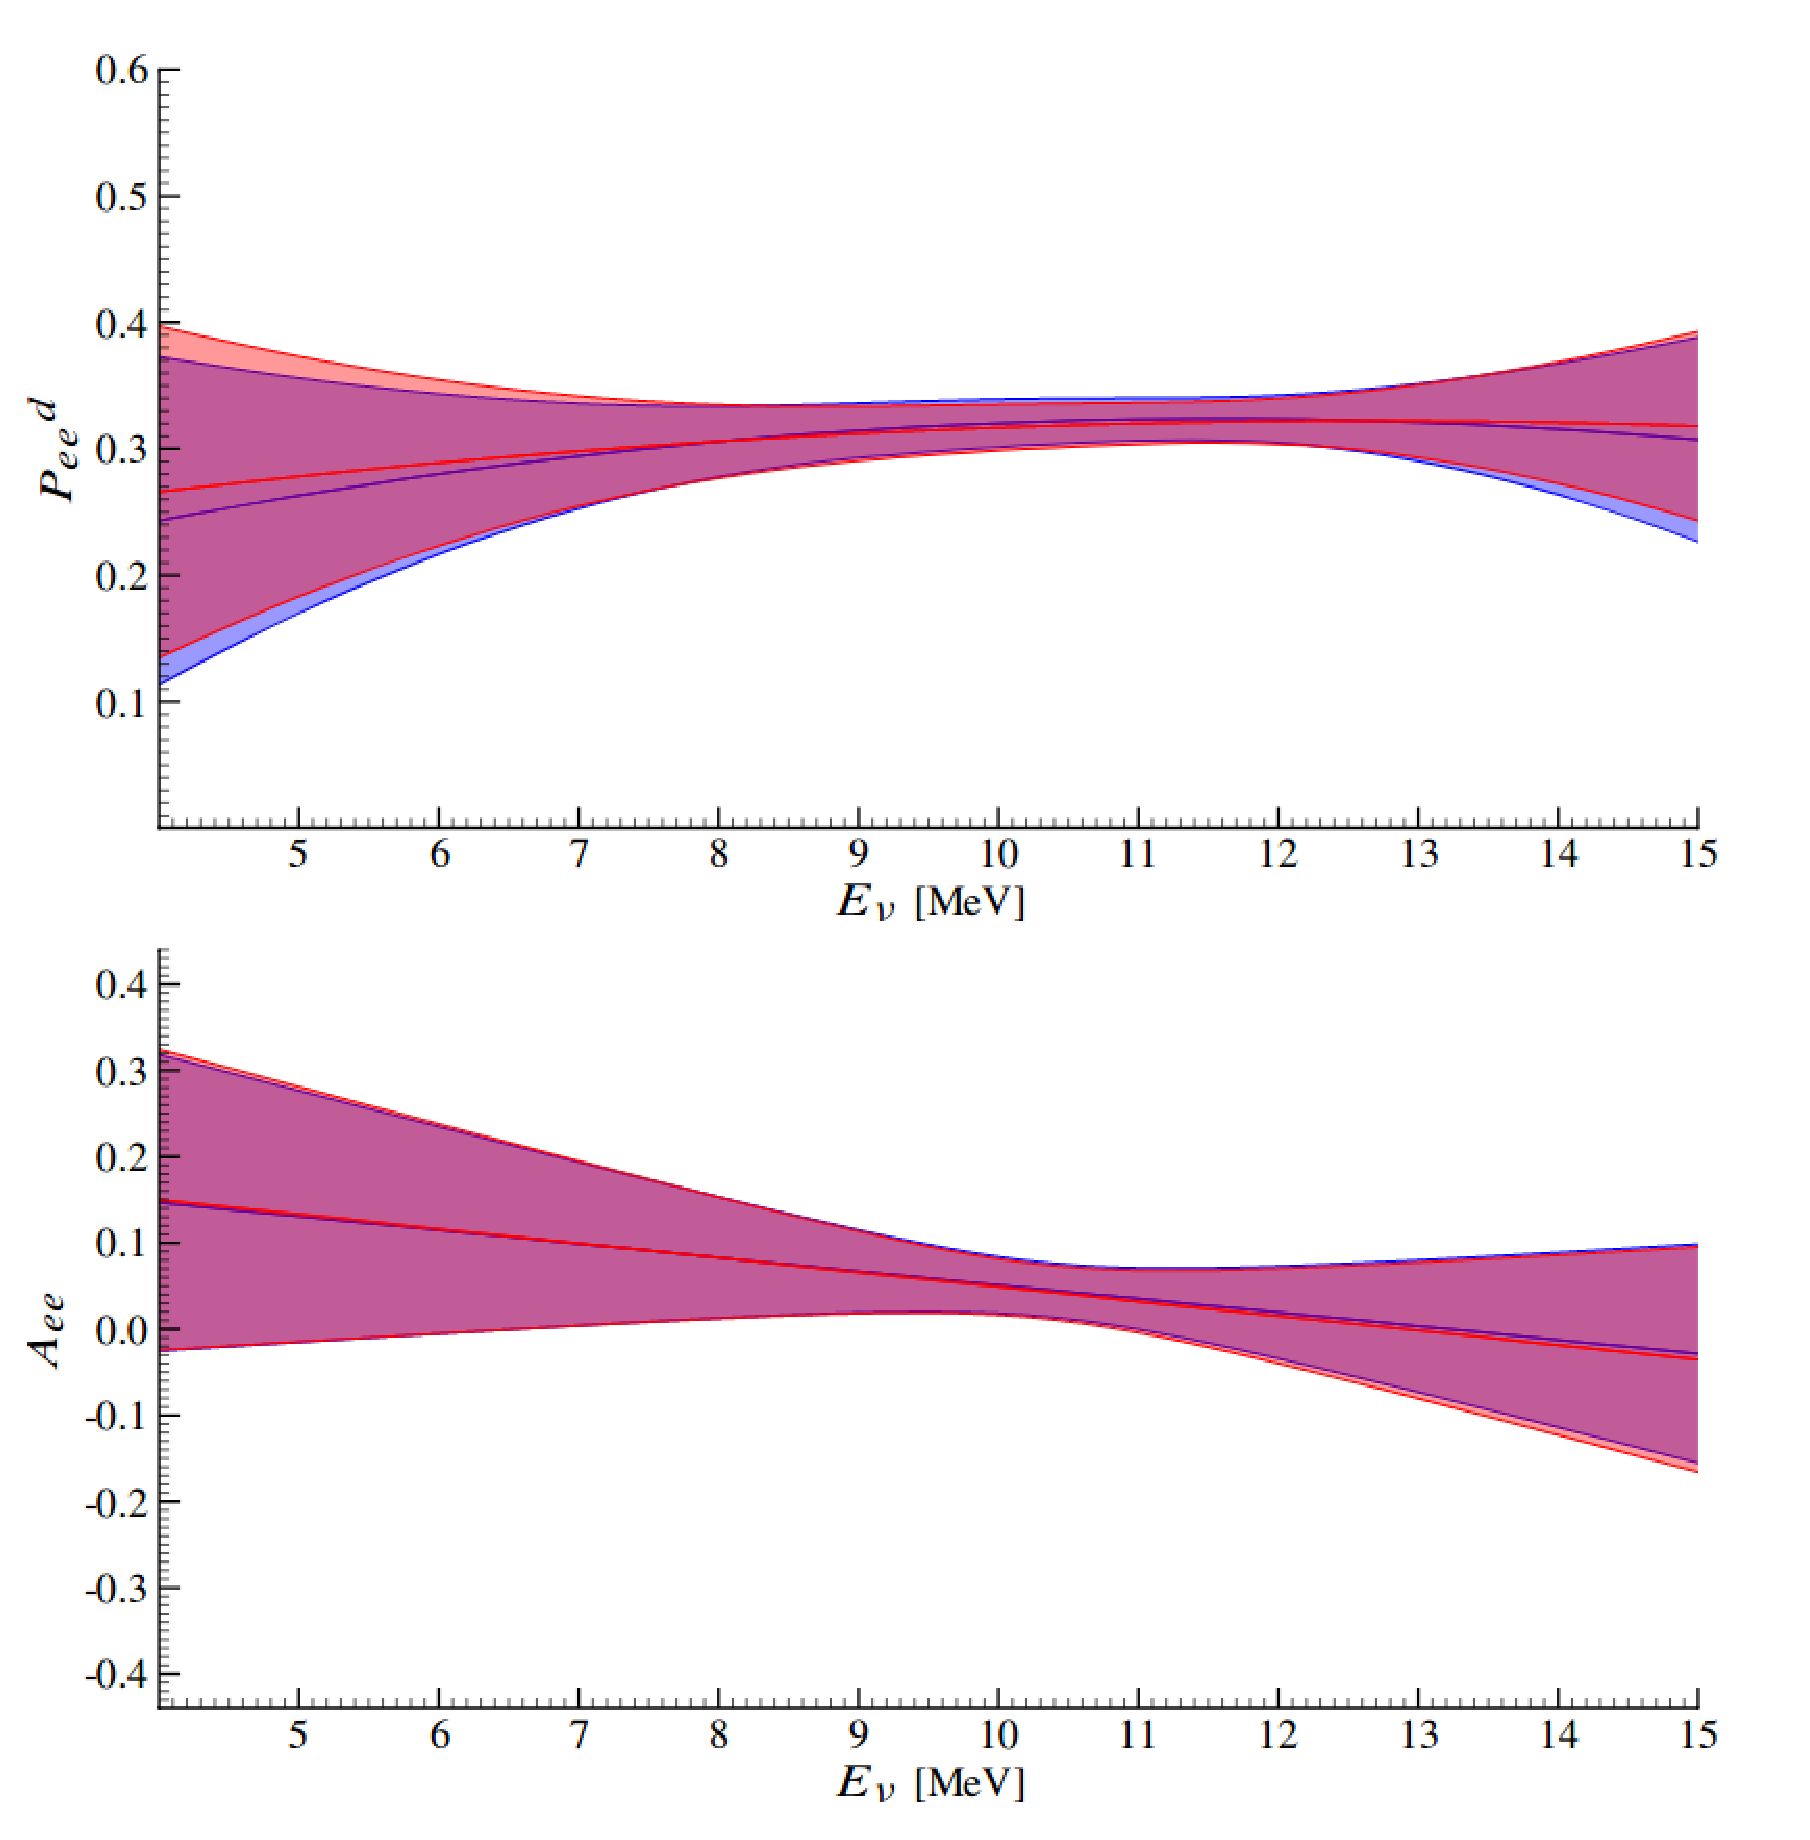
\includegraphics[width=\textwidth]{sno_pee}
        \caption[]{}
        \label{fig:sno_pee}
    \end{subfigure}
    \hfill
    \begin{subfigure}[b]{0.58\textwidth}
        \centering
    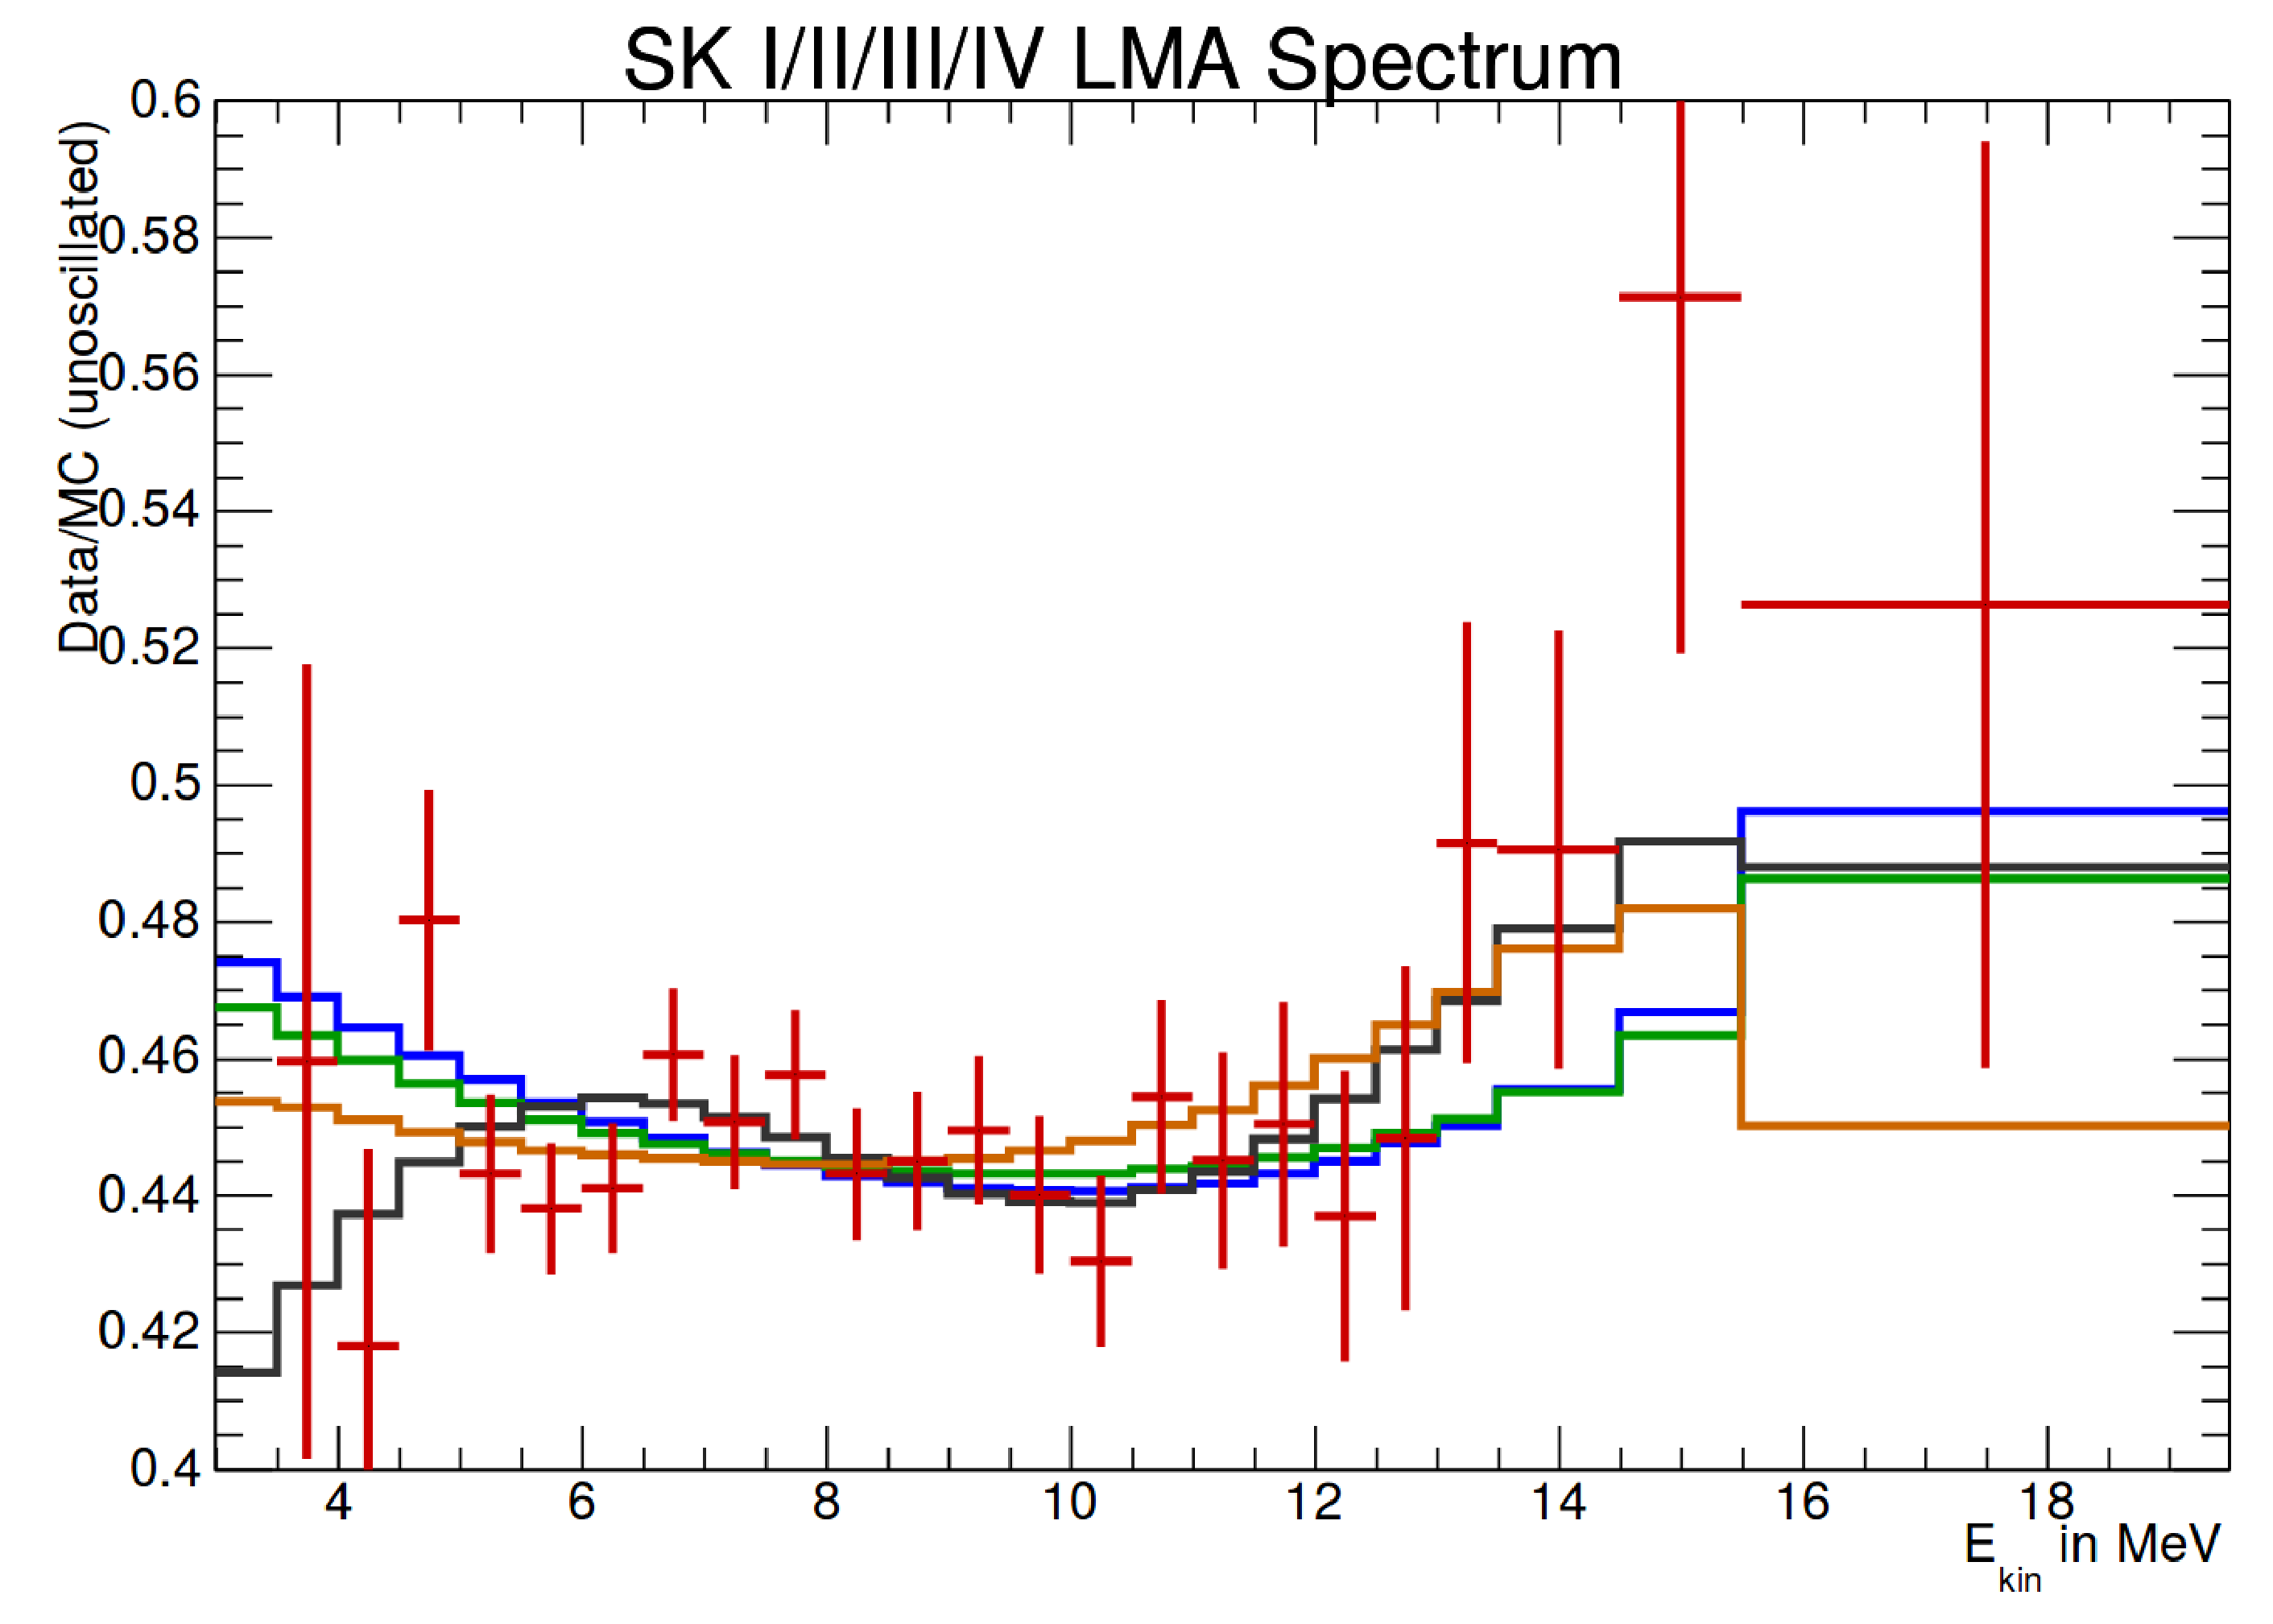
\includegraphics[width=\textwidth]{sk_spectrum}
        \caption[]{}
    \end{subfigure}
    \caption[]{}
    \label{fig:es_b8_measurement}
\end{figure}

Because the ``up-turn'' in the survival probability has not yet been observed,
solar neutrino measurements of $\Delta m^{2}_{21}$ prefer relatively low values
that push the transition region to lower energies.
Using only data from SNO and Super-K the best fit value for 
$\Delta m^{2}_{21}$ is
\begin{equation*}
    \Delta m^{2}_{21} = (4.8^{+1.5}_{-0.8})\times 10^{-5} eV^{2}\text{\citep{superk4}.}
\end{equation*}


In principal, the transition region could be probed as well by a precise
measurement of the survival probability from $pep$ or $\ce{^{7}Be}$ neutrinos.
$pep$ neutrinos are mono-energetic at $E_{\nu}$ = 1.4\,MeV,
this means they should have a survival probability of $53\%$ instead of the
vacuum survival probability of about $56\%$.
$\ce{^{7}Be}$ neutrinos are also mono-energetic at $0.861$\,MeV, providing
them with an expected survival probability of $54\%$.
A measured deviations of these survival probabilities from the expected
vacuum mixing value would provide a measurement of $\Delta m^{2}_{21}$.
But so far measuring these fluxes to that level of precision has not been
possible.
The current best measurement of these neutrino fluxes comes from the Borexino
collaboration~\citep{borexino_nature}, their results are show in Tbl.~\ref{tbl:borexino_results}.
\begin{table}
    \centering
    \begin{tabular} {c| c c}
        & Measured Survival Probability [\%]\\
        \hline
        $pp$ & $56.6 \pm  9.2$\\
        $\ce{^{7}Be}$ & $53.2\pm 5.4$ \\
        $pep$ & $42.8\pm11.4$ \\
    \end{tabular}
    \caption[Borexino Measured Low Energy Survival Probabilities]{
        Measured survival probabilities for low energy solar neutrinos
        from the Borexino experiment~\citep{borexino_nature}.}
    \label{tbl:borexino_results}
\end{table}

The day-night effect also provides sensitivity to $\Delta m^{2}_{21}$.
The smaller $\Delta m^{2}_{21}$ is, the lower the energy threshold is for
neutrinos to experience significant matter effects as they travel through the
Earth.
In practice the day-night effect has been difficult to measure due to
the statistics required to measure a few percent change on the survival
probability.
And so the majority of sensitivity to $\Delta m^{2}_{21}$ for solar neutrino
experiments comes from their ability to measure the transition region.
The day-night asymmetry in the survival probability is often parameterized by the value $A_{ee}$, a value
defined as,
\begin{equation}
    A_{ee}(E_\nu) = \frac{P_{\text{ee, day}}(E_\nu) - P_{\text{ee, night}}(E_\nu)}{P_{\text{ee, day}}(E_\nu) + P_{\text{ee, night}}(E_\nu)}\text{.}
\end{equation}
The SNO measurement of this asymmetry is shown in the bottom panel of~\ref{fig:sno_pee},
they're result is consistent with no asymmetry.
The Super-K measured value for the asymmetry in the observed interaction rate (as opposed to
the survival probability) is
\begin{equation*}
    A_{SK} = (-3.3 \pm 1.0(stat.)\pm 0.5(syst))\%\text{.} 
\end{equation*}

\begin{figure}[htbp]
    \centering
    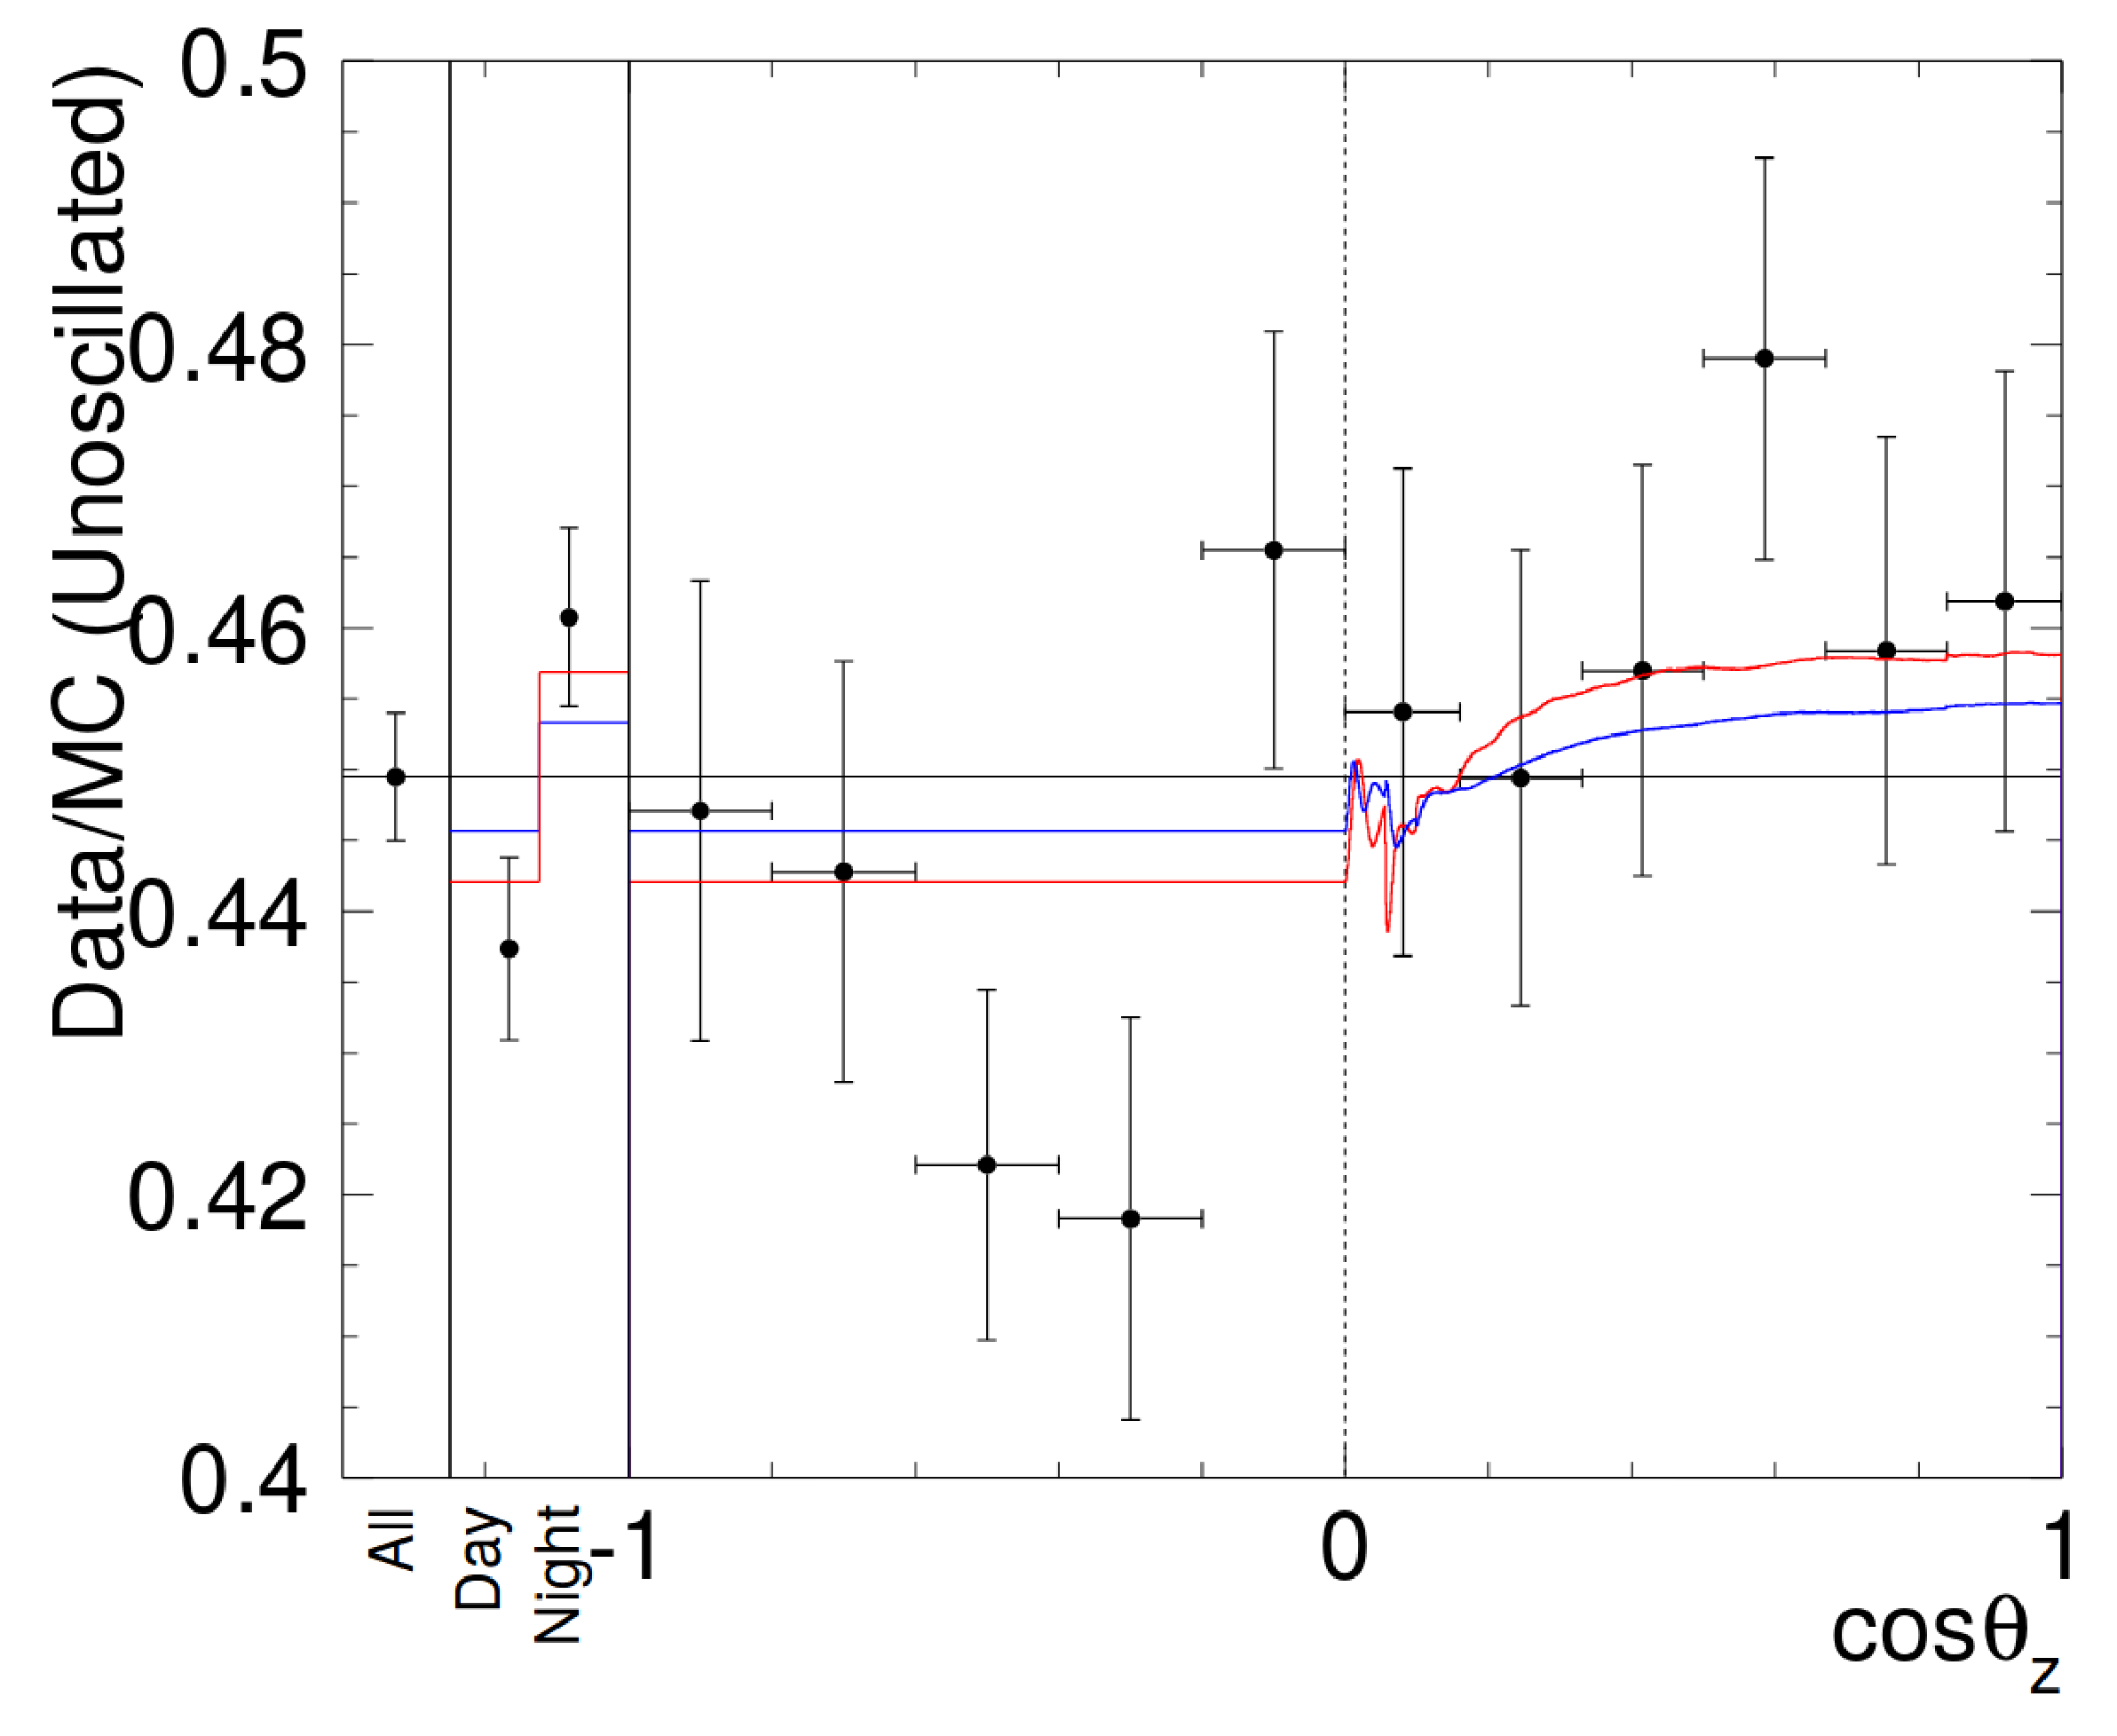
\includegraphics[width=0.65\textwidth]{sk_daynight}
    \caption[Super-K Day Night Asymmetry Measurement]{Zenith angle dependence of elastic scatter interaction rate observed with Super-K. Figure from~\citep{superk4}}
    \label{fig:sk_daynight}
\end{figure}

This value is inconsistent with the no asymmetry at the roughly two-sigma level.
The predicted value for this asymmetry for the best fit KamLAND $\Delta m^{2}_{21}$
is $-1.7\%$ the predicted value for the Super-K+SNO value of $\Delta m^{2}_{21}$ is
$-3.3\%$.%XXX TODO CHECK THIS VALUE
So with relatively small significance, the solar measurement of $\Delta m^{2}_{21}$ from the day-night effect
prefers a lower value than the KamLAND measurement.
Figure~\ref{fig:sk_daynight} shows the Super-K asymmetry measurement in the
observed interaction rate.

\begin{figure}[htbp]
    \centering
    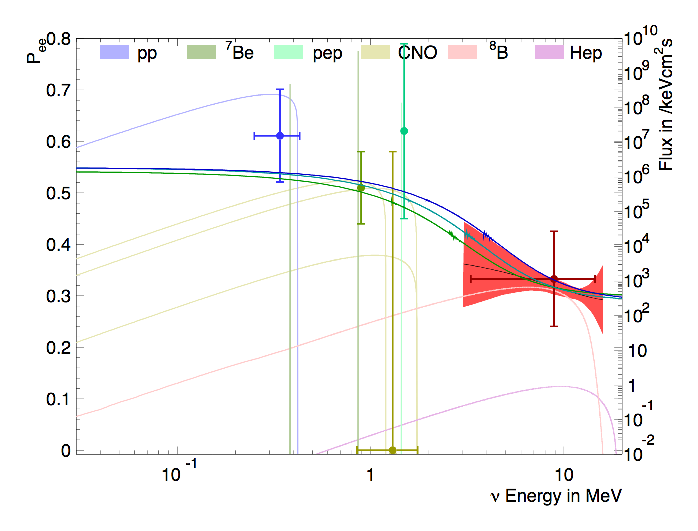
\includegraphics[width=0.78\textwidth]{sk_pee_global}
    \caption[]{Figure from~\citep{superk4}}
    \label{fig:sk_pee_global}
\end{figure}

Figure~\ref{fig:sk_pee_global} shows a summary of solar neutrino measurements
with the solar survival probabilities as predicted by the KamLAND+solar and
the solar only values for $\Delta m^{2}_{21}$.

\begin{figure}[htbp]
    \centering
    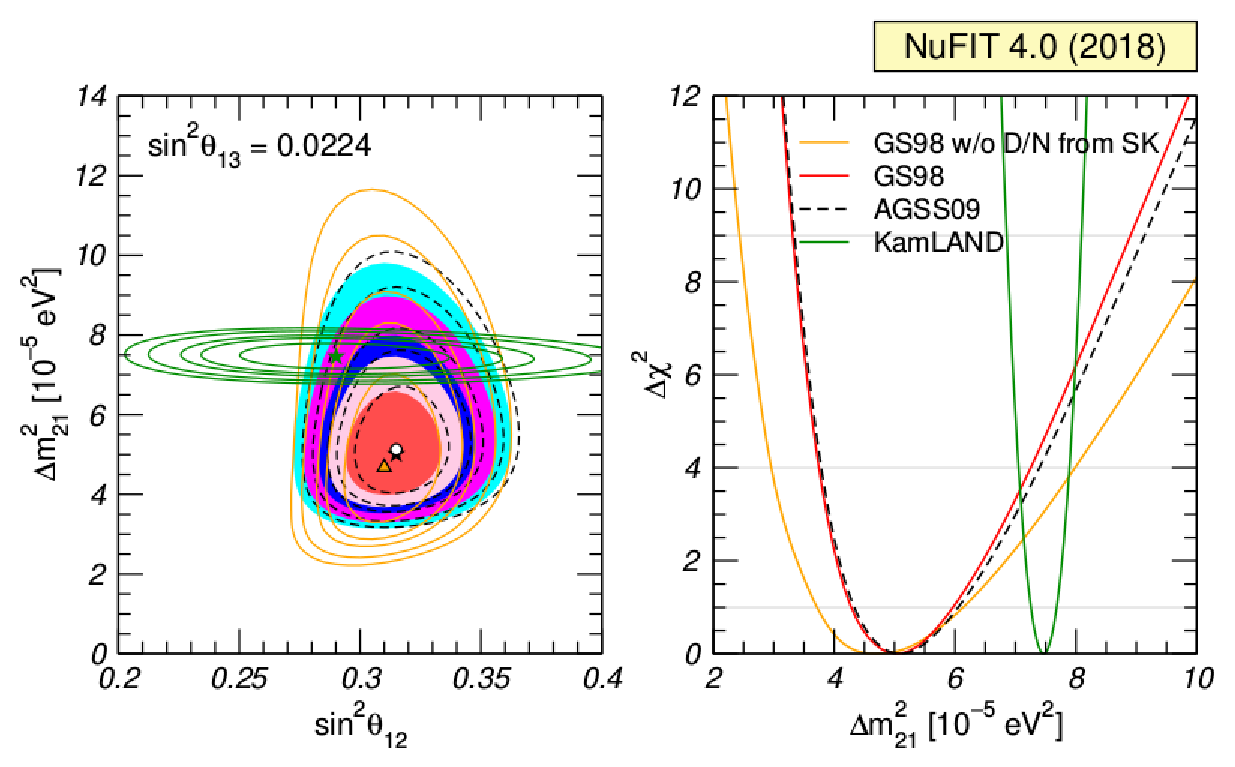
\includegraphics[width=0.78\textwidth]{nufit_dm21_tension}
    \caption[]{Figure from~\citep{nu_fit4}}
    \label{fig:nufit_dm21_tension}
\end{figure}
A global fit for solar neutrino parameters done by Esteban \textit{et. al.}~\citep{nu_fit4},
shown in Fig.~\ref{fig:nufit_dm21_tension},
the overall significance disagreement between the KamLAND+solar and the solar only
measurements for $\Delta m^{2}_{21}$.
They perform a fit to the solar data using solar model input from the GS98 solar abundances
as well as the AGS abundances, and show that uncertainty introduced by the
disagreement in those models is not sufficient to explain the consistently
low value for $\Delta m^{2}_{21}$ observed by SNO and Super-K.
They determine the disagreement between the solar and KamLAND values for
$\Delta m^{2}_{21}$ to have a significance of $\Delta \chi^{2} = 4.7$, or
roughly a $3\%$ chance of being the result of a statistical fluctuation.


\subsection{Non-Standard Interactions}
\label{sec:nsi}
The observed discrepancy in the reactor and solar measured values for $\Delta m^{2}_{21}$
has motivated re-consideration of the models used to predict the solar survival
probability.
It's been shown that if neutrinos produced in the core of the Sun experience
significant flavor sensitive potentials their mixing could be sufficiently modified
to produce results consistent with the observed solar neutrino data, and
the KamLAND measured value for $\Delta m^{2}_{21}$~\citep{richie_nsi,mavans_nsi, nsi_friedland}.
Theories that modify the standard mixing model for neutrinos are generally
referred to as ``Non-Standard Interaction'' or NSI models, because
they often suppose the neutrino might couple to matter in some unexpected way.
Solar neutrinos provide an excellent laboratory for testing NSI models
because solar neutrinos are produced in and travel through matter densities much
higher than what is found in terrestrial neutrino experiments;
similarly solar neutrinos have a much longer baseline than any terrestrial
neutrino sources have.
Additionally, the neutrino production sources within the sun are well
relatively well understood and the Sun's density profile is also well
constrained by solar models.
These two factors allow for NSI theories to produce predictions for solar
neutrino observation that are precise but not ruled out by observations from
reactor, accelerator, or atmospheric neutrino experiments.

Beyond non-standard interactions there exist theories involving sterile neutrinos,
mass-varying neutrinos, neutrino decay, and large magnetic moments, all of
which modify the standard solar neutrino survival probability~\citep{maltoni_solar, richie_nsi}.
Figure~\ref{fig:maltoni_mixing} shows an example of survival probabilities
for a modified up and down quark neutrino interaction and a sterile neutrino
model.

\begin{figure}[htbp]
\centering
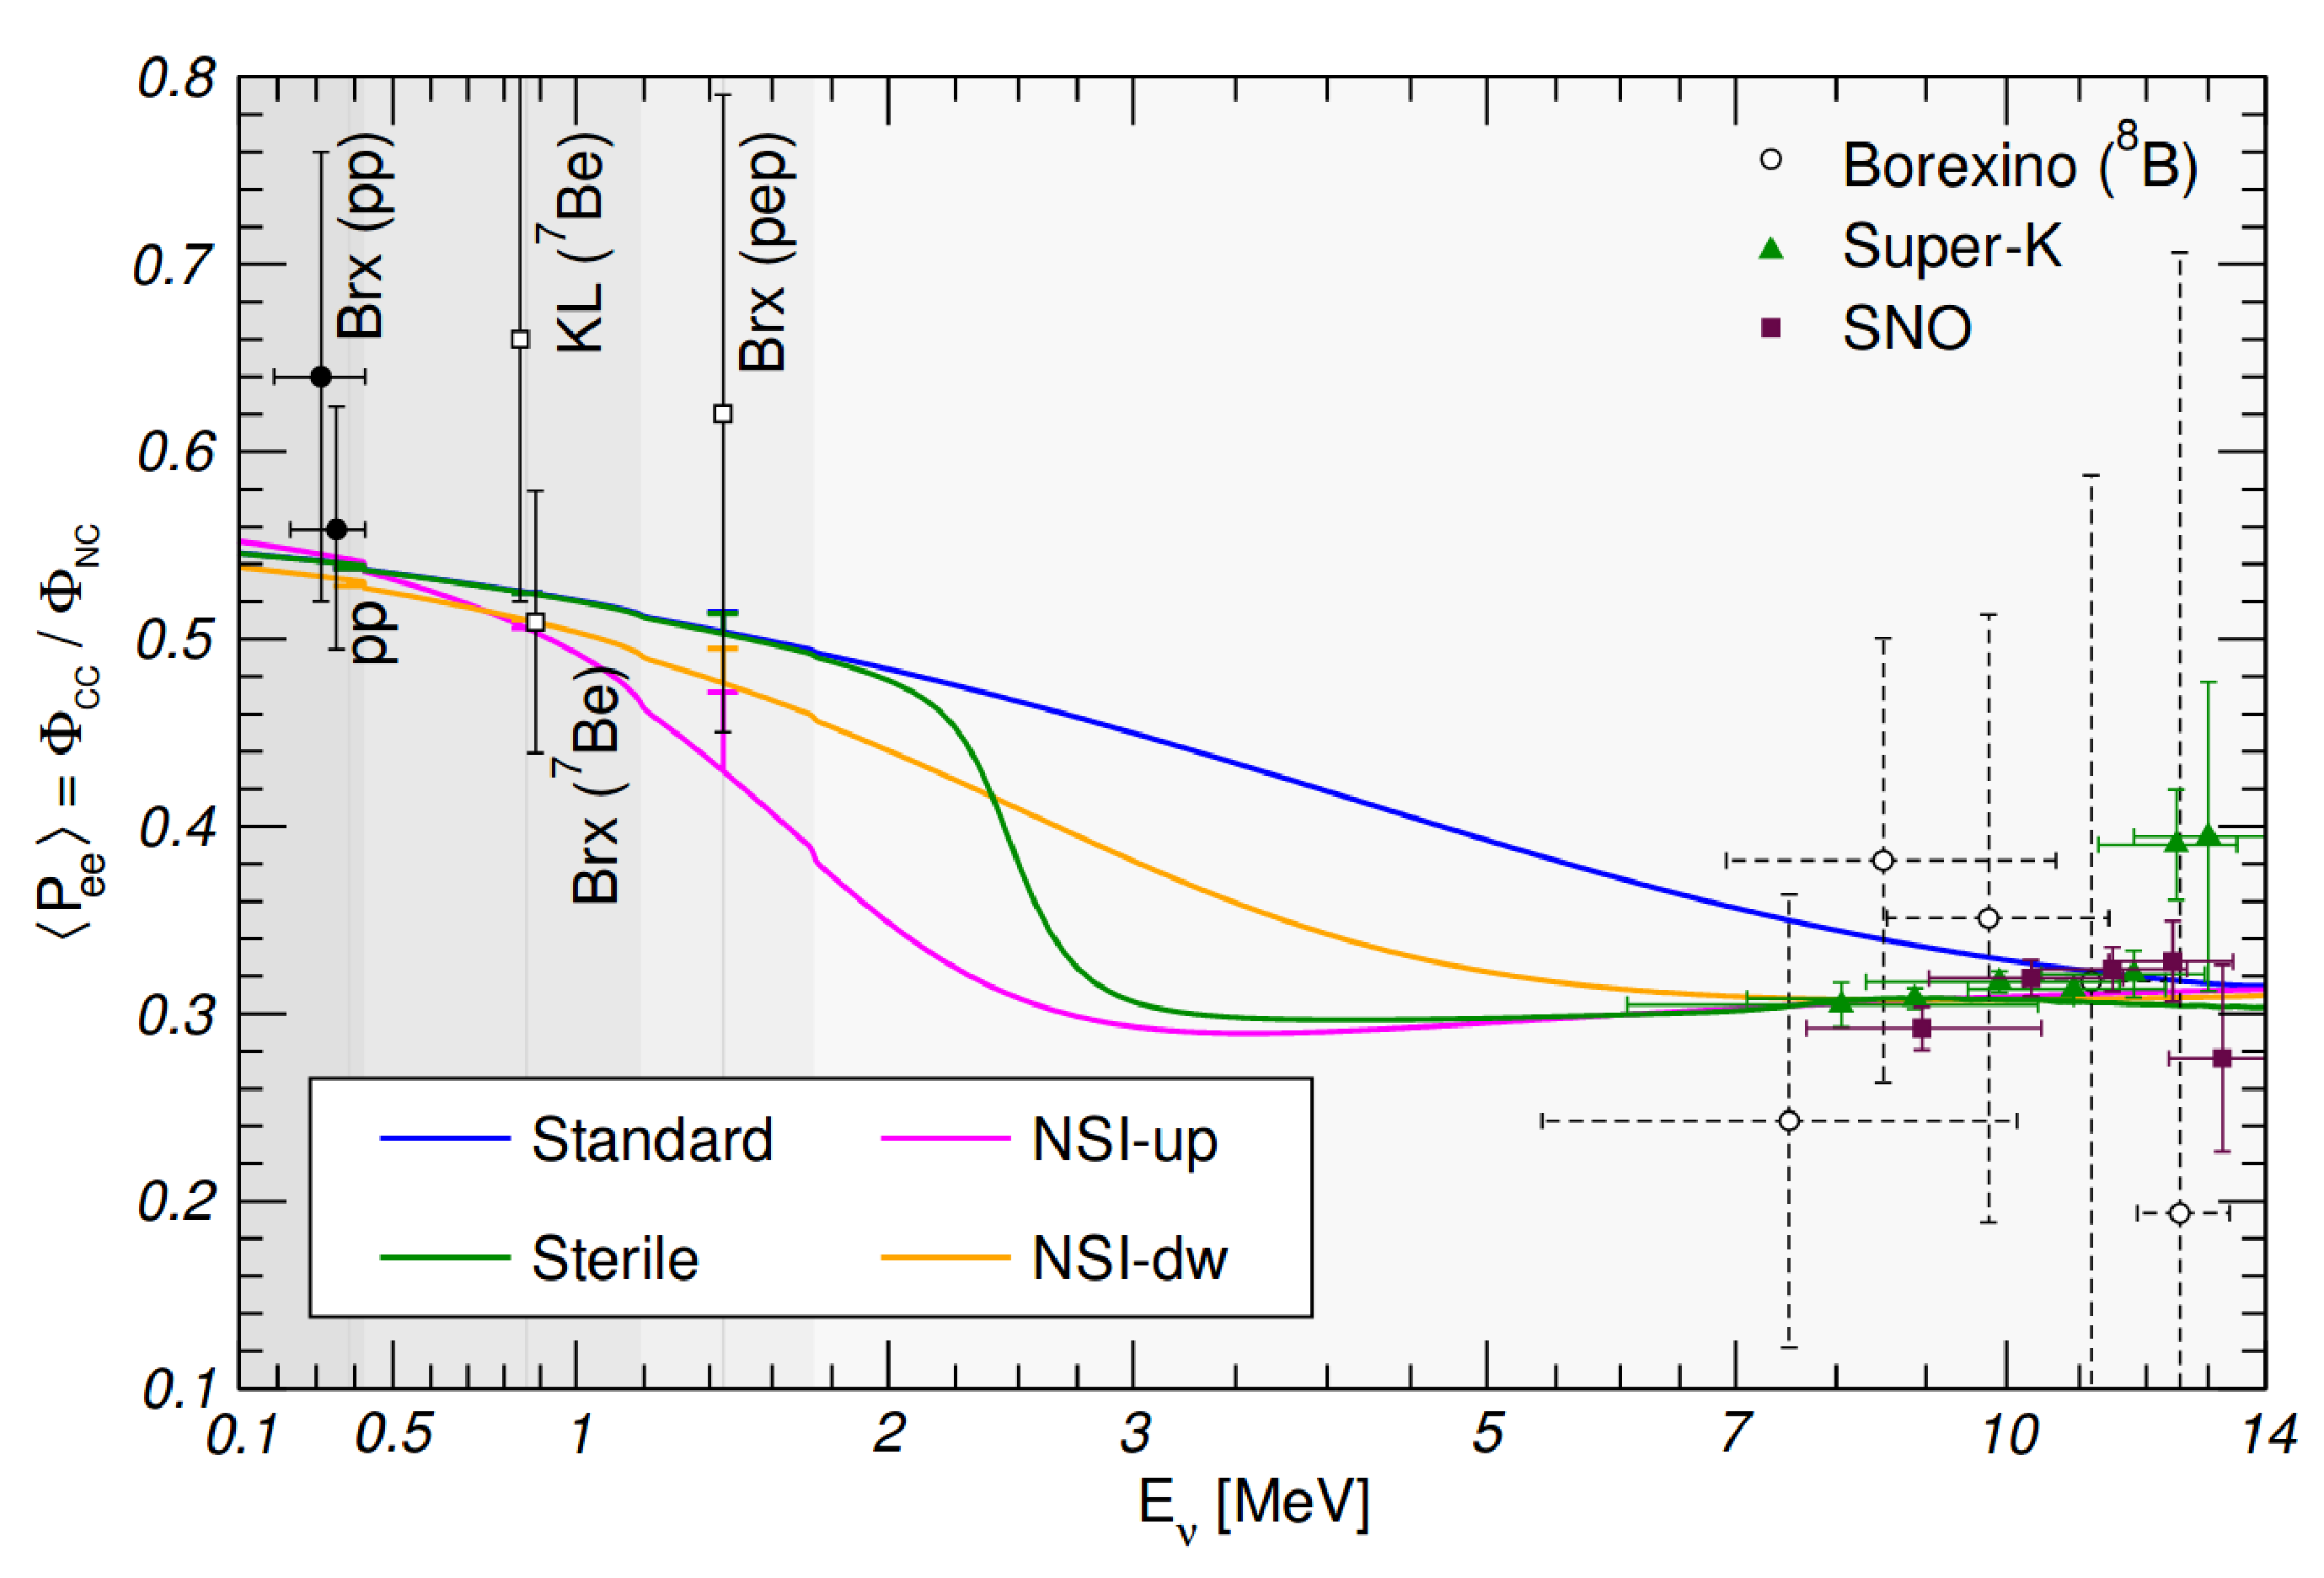
\includegraphics[width=0.68\textwidth]{maltoni_mixing}
\caption[]{Figure from~\citep{maltoni_solar}}
\label{fig:maltoni_mixing}
\end{figure}

\section{Simulation}
Two different simulations of neutrino oscillations were developed to explore the
effects of the modified vacuum mixing potential.
The first
does a full simulation of the neutrino state as it propagates from the
Sun, through the vacuum of space, to a detector at Earth.
Then second calculates the evolution
of the mixing eigenstates for solar neutrinos, and does not simulate individual
neutrinos.
These simulations will respectively be referred to as the ``neutrino'' simulation
and as the ``mass-state'' simulation.
The goal of both simulations is to produce a solar neutrino survival probability
for any given set of standard model mixing parameters and modified vacuum
mixing parameters.
The reason for the two different methods is to allow for different
trade-offs between simulation precision and computational speed.

\subsection{Neutrino Simulation}
For this method of simulation the neutrino state is propagated through the
Sun with its mixing given by
\begin{equation}
    i\frac{d}{dx}\ket{\Psi} = \left[\frac{1}{2E}UM^{2}U^{\dagger} + A_{\mathrm{CC}}\right]\ket{\Psi}\text{.}
    \label{eqn:mixing_schrodinger}
\end{equation}
Where $\ket{\Psi}$ is 3-component vector, each value of which represents
the fraction of the neutrino quantum state in the electron, muon, or tau flavor states,
\begin{equation}
\ket{\Psi} = 
\begin{bmatrix}
    \Psi_{\mathrm{e}}\\
    \Psi_{\mathrm{\mu}}\\
    \Psi_{\mathrm{\tau}}\\
\end{bmatrix}\mathrm{.}
\end{equation}
Since solar neutrinos are all produced as an electron neutrino the
initial state is always
\begin{equation}
\ket{\Psi(x=0)} = 
\begin{bmatrix}
1\\
0\\
0\\
\end{bmatrix}\mathrm{.}
\end{equation}

Given an energy and initial position within the Sun
Eqn.~\eqref{eqn:mixing_schrodinger}
is evaluated numerically using the Runge-Kutta method of numerical integration.
At each step of the integration the neutrinos position is advanced radially
outward a small amount, and using the electron density at the new radius
$A_{\mathrm{CC}}$ is re-evaluated for the next step of integration.
A linearly interpolated solar electron density curve from the BS05OP solar model~\citep{bs_ssm} is used.
This process is repeated until the neutrino reaches a radius where
the solar electron density is near zero and the mixing Hamiltonian is
just standard vacuum oscillations.
The reason the simulation stops there rather than going all the way to the
edge of the sun is because once the matter effect has diminished to a negligible
level, the state of the neutrino no longer evolves it just oscillates around
some central value.
So, upon reaching the end of the simulation the final 5000 neutrino states of the
integration are recorded to provide a full sampling of the possible
neutrino states.
Figure~\ref{fig:sim_example} shows the simulated survival probability of a single
$10$\,MeV neutrino produced in the center of the sun.

\begin{figure}[htbp]
\centering
\begin{subfigure}[b]{0.88\textwidth}
\centering
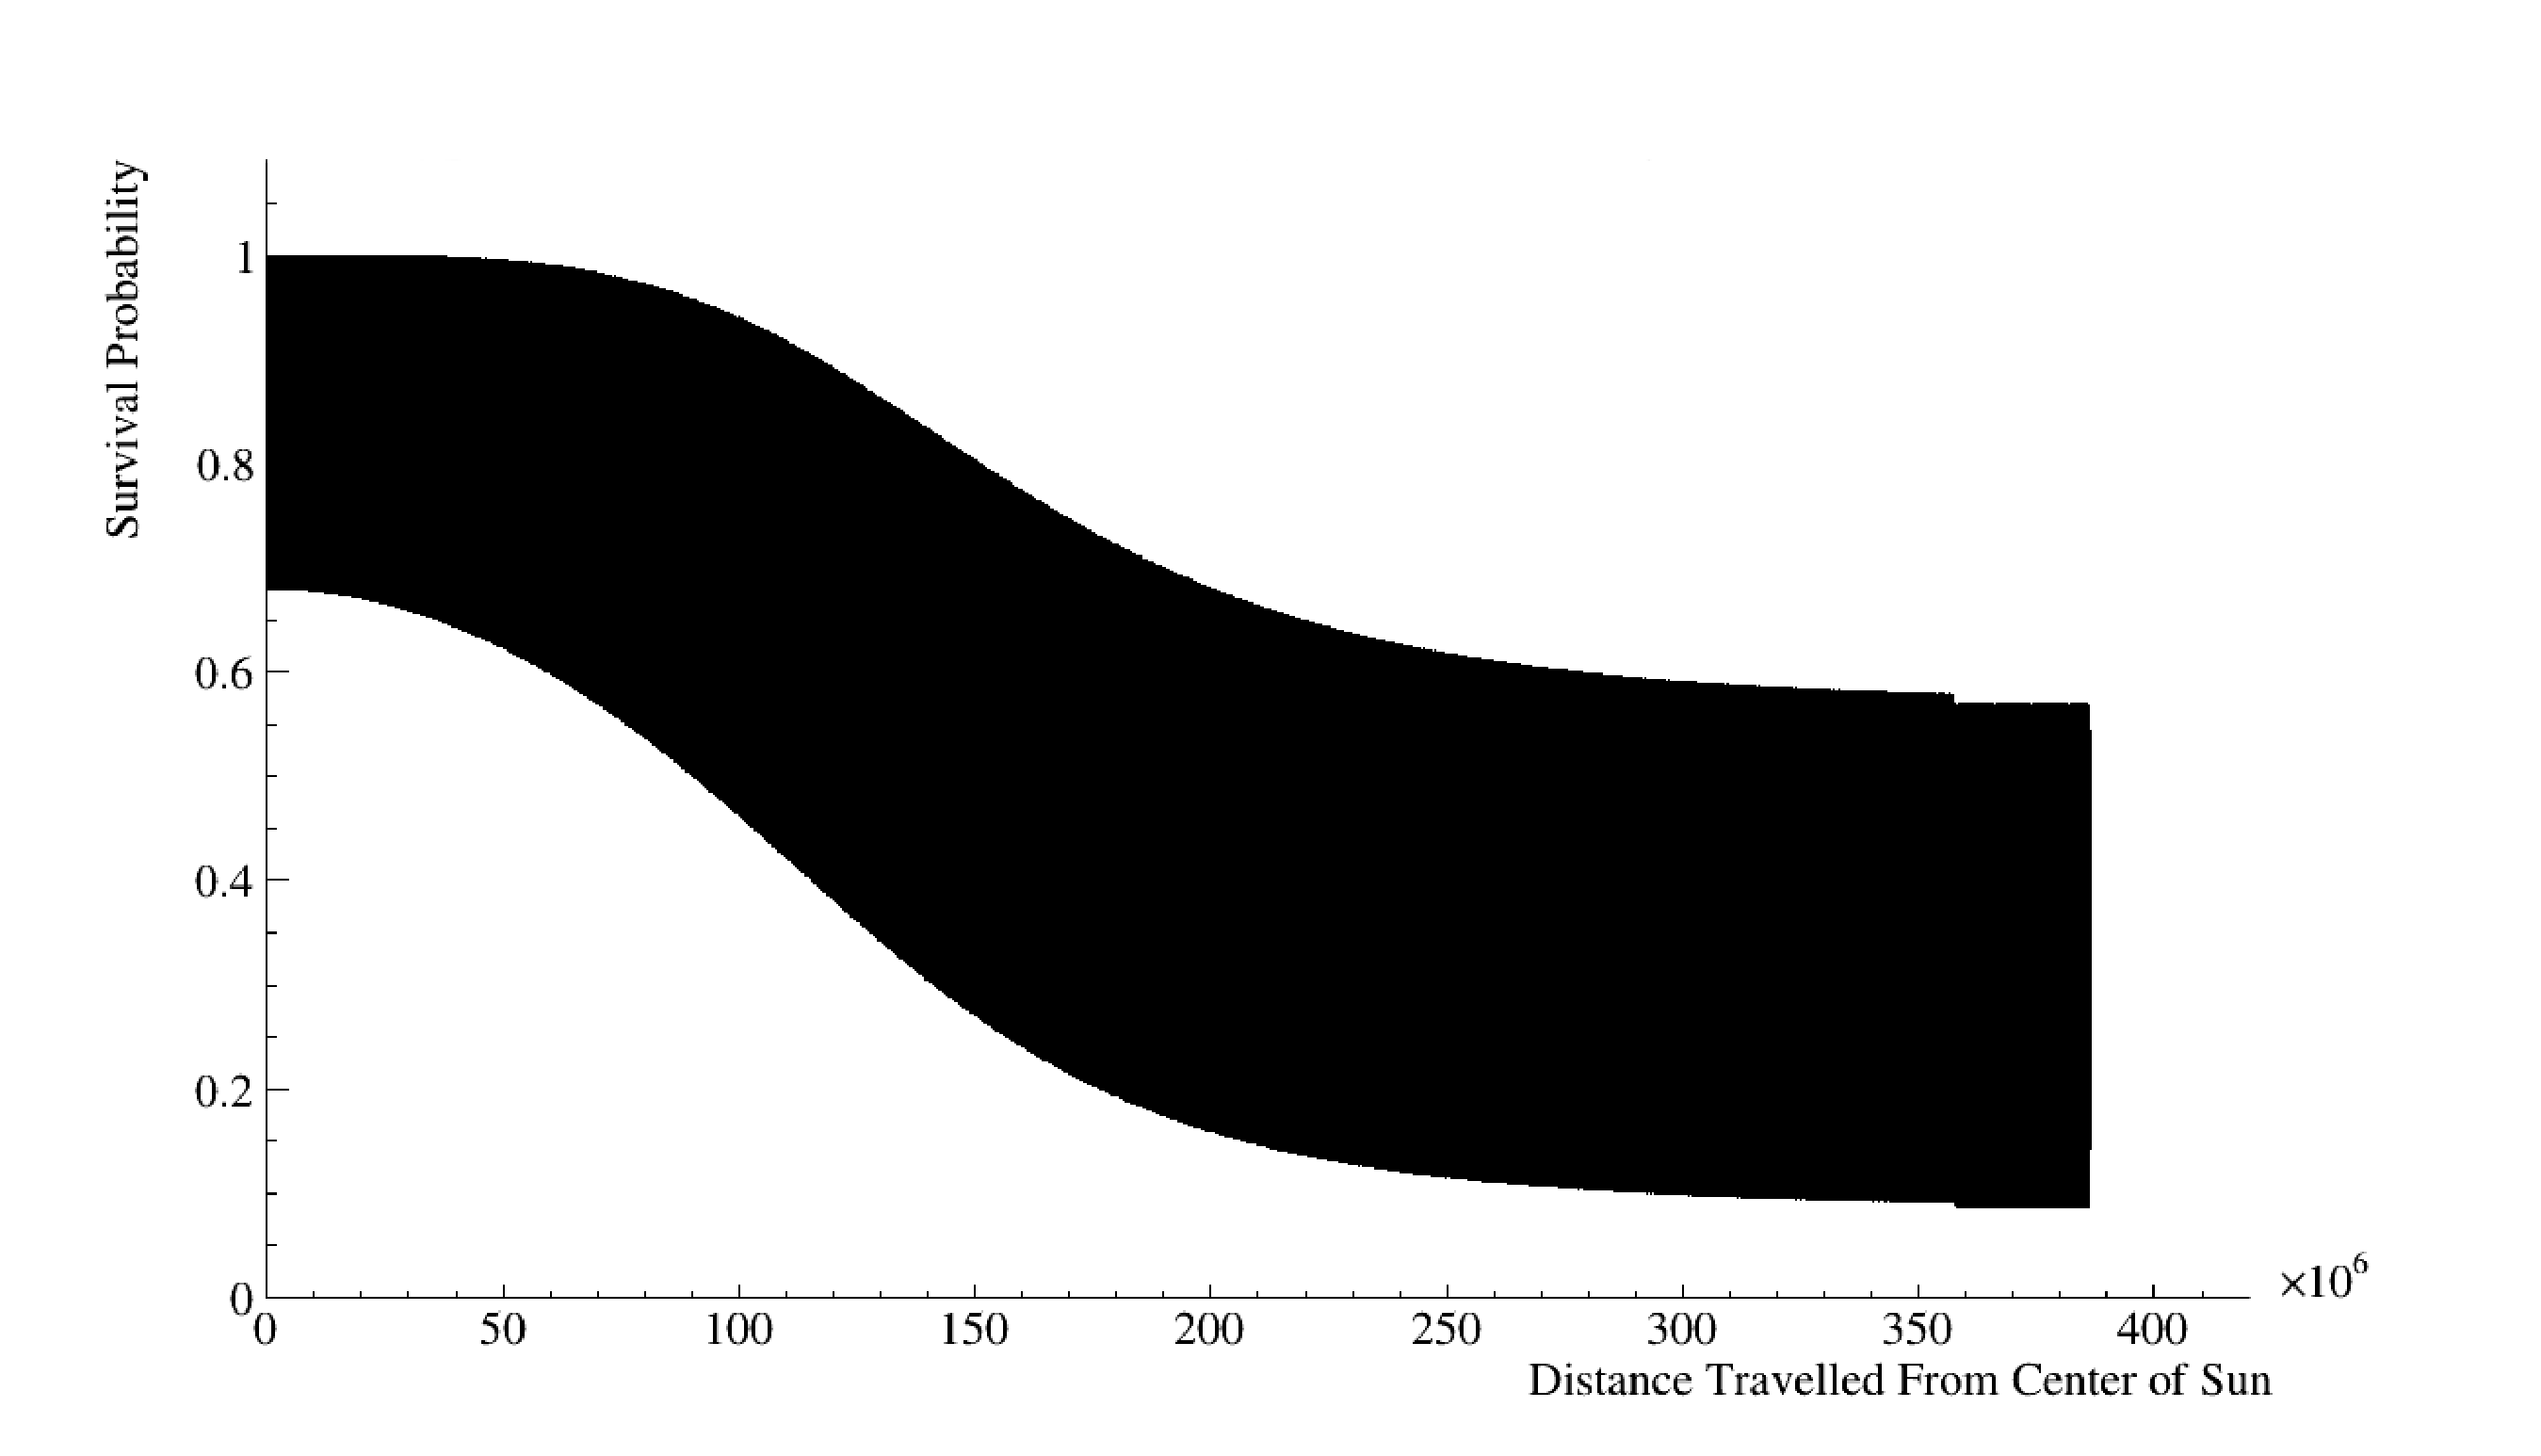
\includegraphics[width=\textwidth]{SolarNeutrino_example.eps}
\caption{}
\end{subfigure}

\begin{subfigure}[b]{0.88\textwidth}
\centering
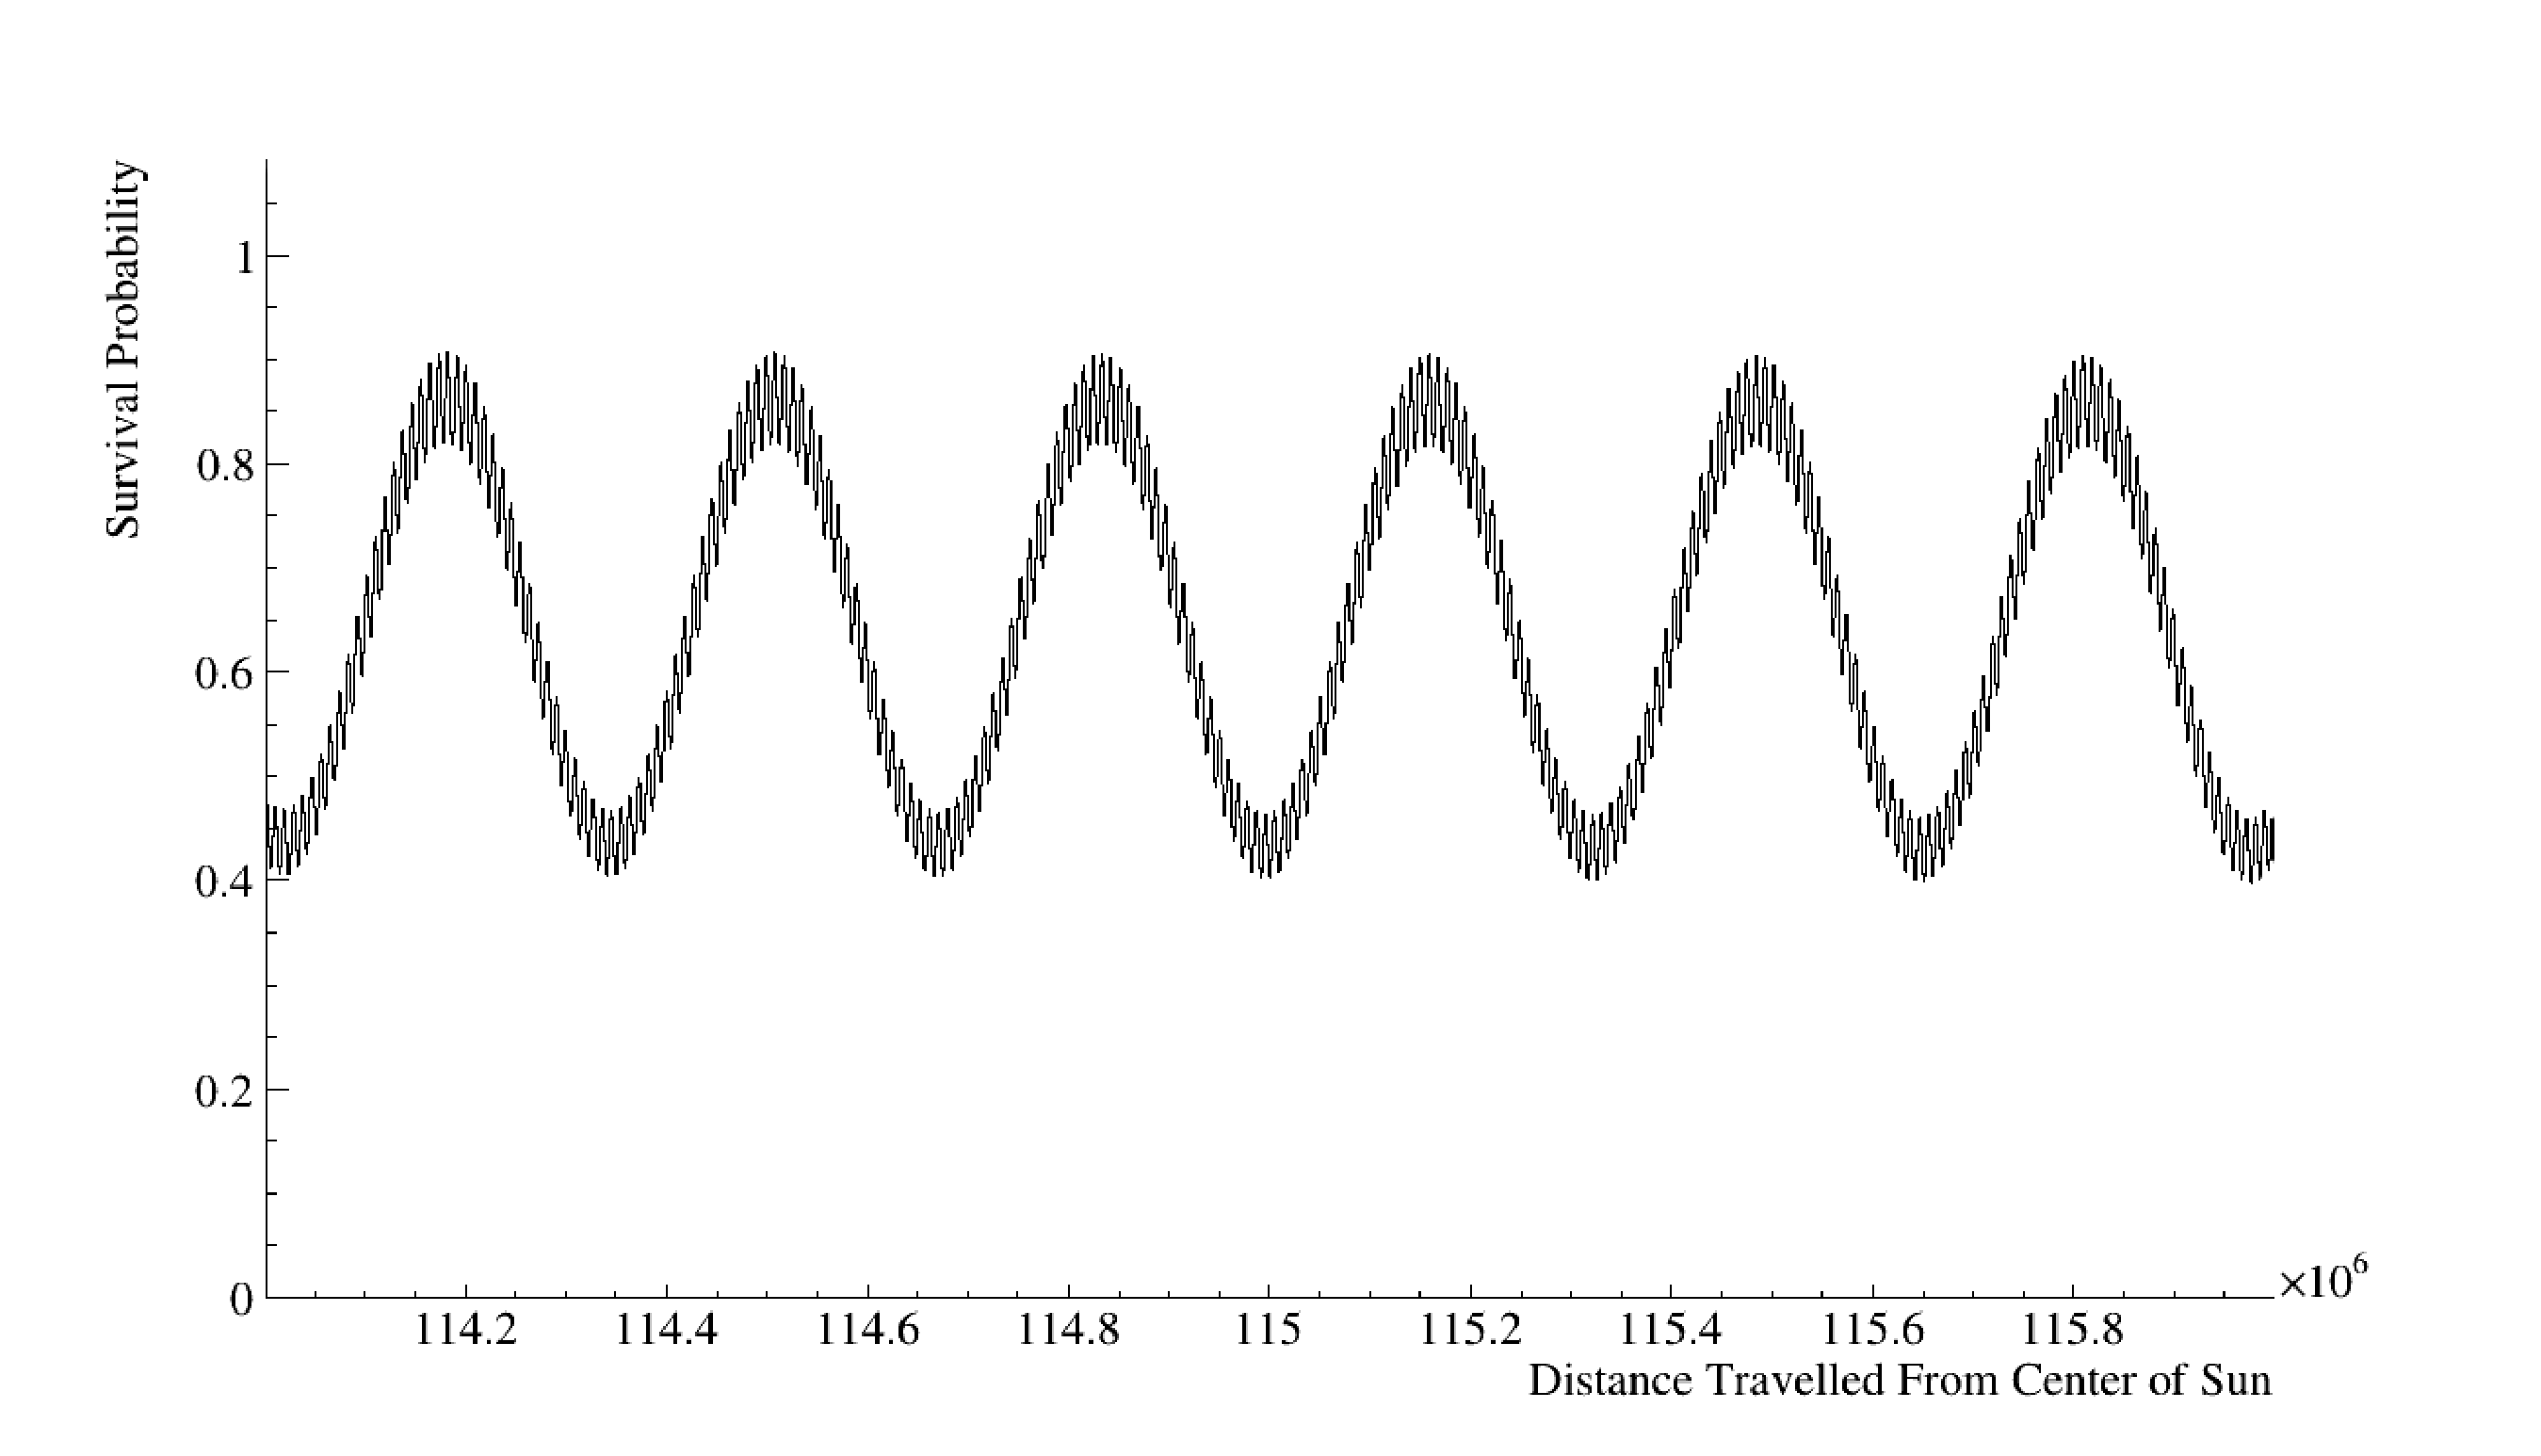
\includegraphics[width=\textwidth]{SolarNeutrino_zoomed_example.eps}
\caption{}
\end{subfigure}
\caption[Example Neutrino State Simulation]{(a) The simulated survival probability for a 10\,MeV solar neutrino produced
in the center of the sun. The bottom panel (b) is the same as the top (a), but zoomed
 in around an arbitrary distance. X-axis units are meters.}
\label{fig:sim_example}
\end{figure}

Simulation was done for 200 neutrino energies spaced logarithmically from
0.1\,MeV to 20\,MeV and for each energy neutrinos at 8192 different starting radii spaced linearly from 0
solar radii to 0.6 solar radii were simulated.
The result of the simulation is approximately 10 billion neutrino states
to provide a representation of all possible neutrino states the sun can produce.
This ``library'' of possible solar neutrino states
is used as input to the modified vacuum potential simulation.

The simulation of neutrinos this way is computationally expensive. A few methods
were explored for ensuring this simulation could be performed in a reasonable
amount of time. The method that was used for nearly all of the results here was
to perform the Runge-Kutta integration on a GPU, which each thread corresponding
to a single sample in energy and production radius.
Even still the production of all the simulated solar states requires approximately
2 GPU-months of processing.
By construction though, the solar simulation is not effected by modified
vacuum potential; the main inputs to the solar simulation are the standard model
mixing parameters and the solar density profile. So, standard model mixing parameters
taken from KamLAND and other non-solar neutrino experiments can be used for
the solar simulation.

%The standard solar survival probability can be calculated as
%$|\bra{\nu_{e}}\ket{\Psi_{\nu}}|^{2}$ for each simulated neutrino and appropriately
%integrating over energies and production radii.
%Since neutrino states are simulated by linearly sampling starting radii and logarithmically
%sampling neutrino energies, states must be weighted by the relevant production
%PDFs in energy and radius.
%Figure~{XXX} shows the standard $\ce{^{8}B}$ survival probability simulated
%this way.

The modified vacuum portion of the simulation is done by first monte-carlo sampling
neutrino energies and production radii, and looking up the simulated
neutrino state that corresponds to the sampled energy \& production radius.
The radial production PDFs for each neutrino type from the BS050P standard
solar model are used for sampling production radii.
The neutrino energy PDFs are also sampled
however, only half of all sample energies are drawn from the relevant production
spectra, the other half are drawn from a uniform distribution across the
relevant energy region.
The motivation for this sampling method is discussed further at the end of
this section.
%This sampling method gurantees that no energy is so poorly sampled 
%that the simulation results are not useful, but also ensure that the most
%well sampled energies are those most typically produced in the Sun.

Since MC sampling produces energy and production radius values that fall
between bins used when producing the solar state library, the states
from the closest available radius bin is used. For energy
a random choice is made between the energy bins immediately above and below
the desired energy is performed, the probability of choosing either bin
is dependent on how close the desired energy is to that bin.
This process is repeated for $1000000$ simulated neutrinos for each solar
neutrino type, \textit{e.g.} $\ce{^{8}B}$, $pep$, etc.

% TODO need typical radii/energy sample counts
Once  monte-carlo samples of solar neutrino states are calculated, the
states are used as inputs to a simulation of the modified vacuum potential.
This simulation is in principle the same as the solar simulation,
it simply involve evaluating Eqn.~\eqref{eqn:mixing_schrodinger}, where 
$A_{\mathrm{CC}}$ is replaced by $A_{\mathrm{vac}}$.
Unlike the solar simulation where the electron density changes,
the value for $A_{\mathrm{vac}}$ is modeled as a constant 
as the neutrino propagates between the Sun and Earth.
The constant value for the Hamiltonian means
Eqn.~\eqref{eqn:mixing_schrodinger} can be evaluated using
a combination of analytic and numerical techniques instead of numerical
integration.

The modified vacuume state evolution done by first evaluating the mixing
Hamiltonian and diagonalizing the resulting matrix.
Diagonalization is done using the GNU Scientific Library~\cite{gsl_ref}
linear algebra routines.
The resulting eigenvectors are used to transform to a basis where the
Hamiltonian is diagonal and the state can be evolved by evaluating
\begin{equation}
\ket{\Psi_{k}(x)} = e^{(-iE_{k}x)} \ket{\Psi_{k}(t=0)}\text{.}
\label{eqn:chameleon_evolution}
\end{equation}
The energy $E_{k}$ is the k$^{\mathrm{th}}$ energy eigenvalue determined by the
diagonalization routine, $\ket{\Psi_{k}}(t=0)$ is neutrino state, in the eigen-basis, at
the time that it enters the modified vacuum potential;
the states from the solar simulation are transformed to the eigen-basis
and used for $\ket{\Psi_{k}(t=0)}$.
Equation~\eqref{eqn:chameleon_evolution} is evaluated for $x=1$AU
and the new state is transformed back into the flavor basis.
Performing this series of steps for each monte-carlo sampled neutrino
state provides the expected distribution of states as they arrive at Earth
having travelled through a modified vacuum mixing potential.

The final step of the calculation is to evolve the sampled neutrino states through
the Earth, to the detector.
This is done similarly to the simulation of neutrino propagation through the
Sun.
The calculation for this is done for only a ``day'' path through the earth
and a ``night'' path. The ``day'' path simulates the neutrino only travelling
through the crust of the Earth. The ``night'' path simulates the neutrino
travelling through the Earth, including the high density core.
The one-dimensional earth density profile is from Ref.~\citep{PREM} is used.
%This results in an simulation of the day-night effect for neutrino oscillation.

The result of this chain of simulation steps is monte-carlo samples
of neutrino flavor states. The survival probability is calculated as,
\begin{equation}
P_{ee}(\ket{\Psi}) = |\braket{\nu_{e}}{\Psi_{nu}}|^2
\end{equation}
for each neutrino state.
Performing an average of survival probabilities binned in neutrino energy 
gives the survival probability as a function of energy $P_{ee}(E_{\nu})$.

Since neutrino states are monte-carlo sampled to calculate $P_{ee}(E_{\nu})$
each value has statistical uncertainty from the number of samples used.
This problem was somewhat exacerbated by the distributions of some of the
solar neutrino energy PDFs having small values in areas that are important for
comparing to solar neutrino data. For example the low energy portion of the
$\ce{^{8}B}$ solar neutrino flux is very important for solar neutrino experiments,
but makes up a relatively small portion of the full $\ce{^{8}B}$ neutrino flux.
To mitigate the problem of large sampling uncertainty for important regions in
solar neutrino energy, energies were sampled according to a flat distribution
and according to the PDFs for each solar neutrino flux. These two methods of sampling
were performed in equal proportions for each flux type.

This method for calculating a modified vacuum survival probability has the
distinct drawback of being computationally expensive, to the point
where it cannot be used in a fit to data.
It does, however, have the benefit of simulating effects from a non-adiabatic
transition from between different potentials that effect neutrino mixing.
Non-adiabatic effects are important because the neutrino is neither produced nor
detected in a vacuum, so for modified vacuum potential to have an effect
that can be detected with a terrestrial detector there must be some
non-adiabatic transition.

\subsection{Mass State Simulation} %TODO better subsection titles
For the mass state simulation instead of simulating individiual neutrino
states, only the eigen-states are simulated.
For each production radius and production energy within the sun the
the mixing Hamiltonian is diagonalized,
\begin{equation}
    H = U M U^{\dagger} + A_{\mathrm{CC}} = P D P^{\dagger}\text{.}
\end{equation}
Where $D$ is a diagonal matrix that gives the effective mass-squared
difference between the mass-states.
$P$ gives the flavor composition of the effective mass states,
$\ket{m_{1}}$, $\ket{m_{2}}$, $\ket{m_{3}}$.

A neutrino produced in an electron flavor state, is given by
\begin{equation}
    \ket{\nu} = \sum_{k=1}^{3}\braket{m_{k}}{\nu_{e}}\ket{m_{k}}\text{.}
\end{equation}
The neutrino state is then evolved adiabatically into a modified
vacuum potential given by
\begin{equation}
    H = U M U^{\dagger} + A_{\mathrm{vac}}\text{.}
\end{equation}
The eigenstates from the modified vacuum Hamiltonian gives the neutrino mass
states $\ket{\mathrm{vac}_{1}}$, $\ket{\mathrm{vac}_{2}}$, $\ket{\mathrm{vac}_{3}}$.
So the neutrino state is now given by
\begin{equation}
    \ket{\nu} = \sum_{k=1}^{3}\braket{m_{k}}{\nu_{e}}\ket{\mathrm{vac}_{k}}\text{.}
\end{equation}
In general this equation could be used to evaluate the
survival probability, as is shown in Section~\ref{sec:neut_osc}.
However, equation~\ref{eqn:pee_adiabatic} shows that this process produces
terms that oscillate as the neutrino state evolves as well as constant
terms.
Solar neutrino experiments are not sensitive to oscillations in the survival
probability because the production of neutrinos is distributed
throughout the core of the Sun, which is many neutrino oscillation lengths
across.
%For any detected neutrino
%it's impossible to say where within the Sun the neutrino was produced.
%Meaning there's no way to estimate how many oscillation lengths any neutrino
%went through while traveling from the Sun to Earth, and so the oscillations
%are effectively averaged over.

% TODO consider adding a wave-packet decoherence arguement here
%The second reason is that mass-states decohere while travelling from the Sun to Earth,
%meaning in a wave-packet treatment of neutrino oscillations the mass-states
%wave packets will have nearly zero overlap.

Because solar neutrino experiments are not sensitive to oscillations in
the survival probability, terms that oscillate can be ignored.
The survival probability to be calculated as
\begin{equation}
    P_{ee} = \sum_{k=1}^{3}\abs{\braket{m_{k}}{\nu_{e}}}^{2}\abs{\braket{\nu_{e}}{vac_{k}}^{2}}\text{.}
\end{equation}

This method for calculating the survival probability relies
on the neutrino entering the modified vacuum potential adiabatically.
Since the mechanism by which the neutrino is sensitive to the local matter
density is not considered here, it's plausible that the modified
vacuum potential ``turns-on'' slowly enough that there's no non-adiabatic
transition.
However, as mentioned earlier, since the solar neutrinos are neither
detected nor created in a vacuum, a non-adiabatic transition is required
for terrestrial neutrino detectors to be sensitive to a modified vacuum
neutrino potential.
For this model that non-adiabatic transition is assumed to be that the
neutrino does not fully transition from being best described
by a modified vacuum state by the time it's detected.
This is plausible because the oscillation length for higher
energy neutrinos is approximately 200\,km, the earth's atmosphere
is approximately the same size~\citep{atmosphere_profile}.
So it could be the case that solar neutrinos, especially at higher
energies, would not oscillate quickly enough to have a average
survival probability best described by the standard oscillation
probability.
For any set of mixing parameters this assumption can be checked using the
more computationally expensive neutrino state evolution simulation.

The benefit of this method for calculating modified vacuum solar survival
probabilities is that it's computationally much faster than the full
neutrino state evolution;
A much wider search of the parameter space for solar neutrino
mixing to be explored.

\section{Data Sets}
To determine solar neutrino and neutrino mixing parameters that is most
consistent with experimental observations, a fit is done to published
experimental results.
Solar neutrino results from SNO~\citep{sno_combined}, Super
Kamiokande~\citep{superk4, superk_first_solar,superk2, superk3},
Borexino~\citep{borexino_final_results,borexino_nature}, GNO~\citep{gallex, gno},
SAGE~\citep{sage}, and Homestake~\citep{homestake} are used.
Solar neutrino fluxes are constrained by the GS98~\citep{gs98} solar abundance calculations.
Reactor neutrino results from Daya Bay~\citep{daya_bay}, KamLAND~\citep{kamland_reactor, kamland_data_release}, RENO~\citep{reno}
are also used to constrain neutrino mixing parameters.
The KamLAND experiment has also published solar neutrino
measurements~\citep{kamland_solar, kamland_b8},
only their reactor neutrino results are used however.
%The KamLAND solar neutrino results are, however, compatible with and
%significantly less constraining than the comparable measurements made by
%Borexino, SNO and Super-K, so the inclusion of those measurements would not
%effect any fit results significantly.

%///////
The experimental results for each experiment are modeled using methods developed
by Richard Bonventre, Anthony LaTorre and Oliviva Wasalski~\cite{richie_thesis}.
For all solar experiments, except for SNO, the expected event rate in each
energy bin over the experiments sensitive energy region is calculated;
for Super-K and Borexino the event rates are calculated in each energy bin.
Event rates are calculated by performing a convolution of the neutrino
flux spectrum with the interaction cross-section relevant for  each experiment
and with the hypothesized neutrino survival probability spectrum
producing a spectrum of observable elastic-scatter electron energies, or
an event rate for nuclear interactions.
For Super-K and Borexino the electron energy spectrum is convolved with a
detector response function to produce expected event rates.
For the Homestake experiment interaction cross-sections from Bahcall~\citep{bahcall_chlorine}
are used.
For the gallium experiments cross-sections for $\ce{^{71}Ge}$ is given by
the SAGE collaboration in Ref.~\citep{sage_xs} and Bahcall~\citep{bahcall_gallium}.

Each experiment provides their own own measurement of detector
related systematic uncertainties, these uncertainties are all treated as independent,
with the exception of the four Super-K datasets.
 Each Super-K dataset has it's own systematic uncertainty associated with,
but each uncertainty is treated as fully correlated across datasets.
Systematic uncertainties are treated as Gaussian, or a bifurcated
Gaussian in the case of asymmetry uncertainties.
Systematics are marginalized over when evaluating the likelihood
of any hypothesized event rate.

For comparison to SNO data, the likelihood of a survival probability can be evaluated
directly without calculating expected event rates.
SNO reports their measurement of the $\ce{^{8}B}$ survival probability as a quadratic
parameterization,
\begin{equation}
P_{ee}(E_{\nu}) = c_{0} + c_{1}(E_{\nu} - E_{0}) + c_{2}(E_{\nu} - E_{0})^2
\label{eqn:sno_quad}
\end{equation}
where $E_{0}= 10\,\mathrm{MeV}$,
and a linear day-night asymmetry
\begin{equation}
A_{ee}(E_{\nu}) = a_{0} + a_{1}(E_{\nu} - E_{0})\text{.}
\label{eqn:sno_linear}
\end{equation}
A procedure recommended in Refs~\citep{sno_leta} and~\citep{sno_combined} is followed.
A fit to of Eqn.~\eqref{eqn:sno_quad} and~\eqref{eqn:sno_linear} is done to the hypothesized the survival probability,
exacting values for $c_{0}$, $c_{1}$,$c_{2}$, $a_{0}$ and $a_{1}$.
The best fit values are compared to the best fit values reported by SNO to
determine a likelihood.

For evaluating the likelihood of the KamLAND result for a set of
mixing parameters and modified vacuum parameters a simple lookup
is done to their published $\Delta \chi^{2}$ map~\cite{kamland_data_release}.
A similar approach is used to evaluate the likelihood the Daya Bay and
RENO reactor neutrino results. 
The hypothesized value for $\theta_{13}$ is compared to each
experiments measured value with uncertainty to extract a likelihood.


\section{Fit And Results}
Taken together these experimental models can be used to constrain
to the modified vacuum solar survival probability allowing up to
11 free parameters: $\Delta m^{2}_{21}$, $\theta_{12}$, $\theta_{13}$,
each of the 5 $pp$-chain solar neutrino fluxes, the combined flux of the
CNO neutrinos, and the two modified vacuum mixing potentials $A_{\mathrm{e}}$
and $A_{\mathrm{\mu}}$.
A full fit to 11 free parameters is however too computationally
expensive given the speed of the modified vacuum simulation.
Instead a 3 parameter fit is done, allowing $\Delta m^{2}_{21}$ and the
two parameters of the modified vacuum mixing potential to vary.
%For future results it's likely the simulation could be sped up to allow for a higher dimensionality search of the likelihood space.

Fitting was performed in a few different manners

%Move this shit to an appendix
%\subsection{Simplified Modified Vacuum Mixing}
%Probing the idea of modified vacuum mixing with the simulation detailed in
%section XXX proved computationally difficult.
%So I explored simplified method for evaluating the likelihood of a modified
%vacuum mixing potential. The simplification was to restrict the modified mixing
%to be equivalent to a change in the effective value for $\Delta m^{2}_{21}$.
%The motivation being that the observed discrepancy between solar neutrino
%experiments and KamLAND was only in $\Delta m^{2}_{21}$, and not in $\theta_{12}$.
%
%To explore this idea one simply can use standard methods for calculating the
%survival probability, but modify them such that all terms are effected by the
%local electron density ($n_{e}$) use a different value for $\Delta m^{2}_{21}$ than the
%terms that are not effected by $n_{e}$.
%This introduces a new parameter into the theory, $\Delta m^{2}_{21}\prime$, the
%effective mass-squared splitting the neutrino experiences in vacuum.
%
%With this modification a fit to solar neutrino data was performed, allowing
%all mixing parameters to vary. If this version of modified vacuum mixing describes
%reality then the best fit value for the matter mass-splitting ($\Delta m^{2}_{21}$) should be
%consistent with the value determined by KamLAND.\@ The value for the vacuum mass
%splitting ($\Delta m^{2}_{21}\prime$) has no-apriori preferred value but it would
%be sensible for it to be near the standard best fit value for $\Delta m^{2}_{21}$
%as determined by solar neutrino only measurements.
%
%The fit to data was performed using a Markov-chain Monte-Carlo method to sample
%the likelihood space of mixing parameters as well as solar neutrino fluxes.
%Figure XXX shows the results of the MCMC sampling. Marginalizing over all
%the mixing parameters, including $\Delta m^{2}_{21}\prime$, gives the best fit
%value for $\Delta m^{2}_{21}$ in matter and the error on it.
%The marginalized result is shown in Figure XXX, the preferred value
%for $\Delta m^{2}_{21}$ from solar experiments is $XXX\pm XXX$, only slightly higher than
%the preferred value in a standard mixing formulation, $XXX$, but still significantly
%lower than the best fit KamLAND value, $XXX$.
%The tension between the solar and KamLAND values of $\Delta m^{2}_{21}$ is at
%the $XXX\sigma$ level in the standard formulation, this version of modified
%vacuum mixing reduces that to $XXX\sigma$, at the cost of introducing a new
%parameter into the theory.
%
%The improvement in agreement between solar neutrino experiments and KamLAND on
%the value of $\Delta m^{2}_{21}$ is not large enough to constitue compelling evidence
%that this simple version of modified vacuum mixing describes reality much better
%than standard mixing. And so this motivates going back to a fuller description
%of modified vacuum mixing, that allows for a fuller description of how
%neutrinos might oscillate between the Sun and Earth.
